\documentclass[12pt]{article}
\usepackage[utf8]{inputenc}
\usepackage[dutch]{babel}
\usepackage[rightcaption]{sidecap}
% \usepackage{minted}
\usepackage{graphicx}
\usepackage[colorlinks=true, allcolors=blue]{hyperref}
\usepackage{sectsty}
\usepackage[paperheight=29.7cm,paperwidth=21cm,textwidth=15cm]{geometry} %A4 size
\usepackage{fancyhdr}
\usepackage[siunitx]{circuitikz}
\usepackage{tabularx}
\usepackage{physunits}
\usepackage{booktabs}
\usepackage{tikz}
\usepackage{pgfplots}
\usepackage{karnaugh-map}
\usepackage[nocompress]{cite}
\usepackage{cite}
\usepackage{parskip}
\usepackage{amsmath,amssymb,amsfonts}
\usepackage{algorithmic}

% The preceding line is only needed to identify funding in the first footnote. If that is unneeded, please comment it out.
\usepackage{textcomp}
 % More defined colors
% We will externalize the figures



% Footers/Headers opmaak:
\pagestyle{fancy}
\lhead{}
\chead{\textit{Practicum 4: Digitale Techniek - Combinatorische logica en geheugenelementen 
}}
\rhead{}
\lfoot{\textit{Semih Can Karakoç}}
\cfoot{\textit{\today}}
\rfoot{\textit{\thepage}}
\renewcommand{\headrulewidth}{0.1pt}
\renewcommand{\footrulewidth}{0.4pt}

% Afbeelding settings:
\graphicspath{ {./Figures/} }
% \sectionfont{\left}
% \subsectionfont{\centering}
% \subsubsectionfont{\centering}

% Voorpagina opmaak:
\title{\textbf{Practicum 4: Digitale Techniek - Combinatorische logica en geheugenelementen }}
\author{\textit{Semih Can Karakoç (695258)}}
\date{\textit{\today}}

% Begin document
\begin{document}

\clearpage\maketitle    % Pas opmaak toe aan voorpagina
\thispagestyle{empty}  % Haal page number weg
% Voorpagina plaatje:
\begin{figure}[h]
    \centering
    % \includegraphics[width=0.6\textwidth]{ELEKTRA.png}
\end{figure}
\pagebreak

\tableofcontents    % Inhoudsopgave
\pagebreak

\section{Inleiding}
Tijdens dit practicum is er geëxperimenteerd en onderzocht naar de werking van de multiplexer, BCD-encoder en ringtellers.
Het doel van dit practicum is dan ook om de aspecten van deze logische functies te begrijpen en in de praktijk toe te kunnen passen.
Om de bovenstaande practicumdoel te behalen zijn er in totaal vier experimenten uitgevoerd. 
Daarbij zijn de bijbehorende deelopdrachten uitgewerkt in dit verslag. 

Dit verslag gaat in op de volgende onderwerpen: 
\begin{enumerate}
    \item Logische schakelingen lezen, bouwen en ontwerpen;
    \item Binary Coded Decimal (BCD);
    \item 4-bit multiplexer;
    \item D-flip-flops en J-K-flip-flops;
    \item Ringtellers;
    \item Waarheidstabellen;
    \item Booleaanse algebra.
\end{enumerate}
\vspace{9cm}
NOTE: \textit{alle getekende logische schakelingen in dit verslag zijn zelf gemaakt met draw.io!}
\pagebreak
\section{Probleem- en doelstelling}
\label{Problem}
Dit verslag bevat de volgende probleemstelling:
\begin{itemize}
    \item \textit{``Inzicht krijgen in de werking van een aantal complexe logische schakelingen en daarna deze op een efficiënte wijze te ontwerpen en te bouwen?''}
\end{itemize}
\vspace{0,5cm}
De volgende doelstellingen behoren tot dit practicum:
\begin{enumerate}
    \item Inzicht te verkrijgen in logische functies die ten grondslag liggen aan de digitale techniek;
    \item Waarnemingen te verrichten aan de bijbehorende eenvoudige logische schakelingen;
    \item De bijbehorende meetgegevens en waarheidstabellen op een juiste wijze te verkrijgen en te interpreteren;
    \item De vergaarde gegevens te verwerken tot een verslag.
\end{enumerate}

\vspace{0,5cm}
Aan het einde van dit verslag onder het kopje \ref{Conclusie}:\textit{``Conclusie''} zal de gestelde probleemstelling beantwoord worden.
\pagebreak

\section{Practicumbenodigdheden}
\label{practicumbenodigdheden}
Hieronder zijn de benodigdheden op een rijtje gezet die nodig waren voor het uitvoeren van het practicum:
\begin{enumerate}
    \item Digiboard: het 3910 digiboard is een bord waarop je gemakkelijk de logische schakelingen kan bouwen door gebruik te maken van de ingebouwde poorten. Deze hebben we gebruikt tijdens het practicum.\cite{hps-systemtechnik_ds_DIGI};
    \item Verbindingssnoeren: deze snoeren zijn nodig om verbinding te maken tussen allerlei elektronische componenten; 
    \item Draw.io: dit is een online website waarmee je gemakkelijk logische schakelingen kunt ontwerpen;
\end{enumerate}
\pagebreak

\section{Theoretisch kader}
\label{Theoretisch kader}
\subsection{De basispoorten}
In de digitale techniek zijn er drie belangrijke basispoorten, namelijk:
\begin{enumerate}
    \item De AND-poort: de AND-poort voert een vermenigvuldiging uit tussen de inputs. Dit betekent dat de AND-poort alleen `1' terug geeft wanneer de alle inputs ook `1' zijn, want een vermenigvuldiging met '0' geeft altijd '0' terug. Dit wordt uitgedrukt als: $A \cdot B$;
    \item De OR-poort: de OR-poort voert een optelling uit tussen de inputs. Dit betekent dat de OR-poort alleen `1' terug geeft wanneer minimaal een van de twee inputs `1' is, want een optelling met '1' en '0' is altijd '1'. Dit kan worden uitgedrukt als: $A + B$;
    \item De NOT-poort: de NOT-poort voert een inversie uit op de input. Dit betekent dat de NOT-poort altijd het tegenovergestelde van de input terug zal geven. Een voorbeeld is: $A$ wordt $\overline{A}$ (A niet) \cite{electricalengineering123}.
\end{enumerate}
\subsection{Waarheidstabellen}
Tijdens het practicum wordt ook gebruik gemaakt van waarheidstabellen. 
Een waarheidstabel is een tabel die overzicht geeft over alle mogelijke combinaties van inputwaarden en de bijbehorende uitvoerwaarden \cite{truth2}. 
De waarheidstabel begint aan de linkerkant met de inputwaarden. 
Nadat alle inputwaarden zijn genoteerd komen er twee verticale strepen. 
Deze twee strepen geven aan dat de daarop volgende variabelen uitvoerwaarden zijn \cite{truth1}.  

Zie hieronder een voorbeeld van een waarheidstabel die twee inputwaarden heeft: `A' en `B', en één uitvoerwaarde heeft, namelijk: `$A \cdot B$' (AND-operatie). 
Met deze waarheidstabel kun je alle mogelijkheden overzichtelijk terug zien.
\begin{displaymath}
    \begin{array}{|c|c||c|}
    A & B & A \cdot B \\
    \hline 
    1 & 1 & 1 \\
    1 & 0 & 0 \\
    0 & 1 & 0 \\
    0 & 0 & 0
    \end{array}
    \end{displaymath}
\pagebreak
\subsection{Wetten van de Booleaanse algebra}
In de Booleaanse algebra zijn er een aantal belangrijke wetten die je kunt toepassen om Booleaanse expressies te kunnen vereenvoudigen, namelijk:
\begin{itemize}
    \item Associativiteit: $A+(B+C) = (A+B)+C$ en $A\cdot(B\cdot C) = (A\cdot B)\cdot C$; 
    \item Commutativiteit: $A+B = B+A$ en $A\cdot B = B\cdot A$;
    \item Absorptie: $A+(A\cdot B) = A$ en $A \cdot (A+B) = A$;
    \item Complement: $A + \overline{A} = 1$ en $A \cdot \overline{A} = 0$;
    \item Distributiviteit: $A+(B\cdot C) = (A+B)\cdot (A+C)$ en $A \cdot (B+C) = (A\cdot B)+(A\cdot C)$;
    \item Idempotentie: $A + A = A$ en $A \cdot A  = A$;
    \item De Morgan: $\overline{A \cdot B} = \overline{A}+\overline{B}$ en $\overline{A + B} = \overline{A} \cdot \overline{B}$;
    \item Redundantie: $A\cdot B + A\cdot \overline{B} = A$ en $A\cdot \overline{B} + B = A + B$
    \item Dubbele negatie: $\overline{\overline{A}} = A$ \cite{weyt}.
\end{itemize}
% \subsection{Karnaugh diagram}
% In de Booleaanse algebra moet je vaak een SOP (Sum Of Products) of een POS-expressie (Product Of Sum) opstellen. Deze expressies zijn meestal nog niet vereenvoudigd tot een minimale expressie. 
% Het minimaliseren van een SOP of een POS-expressie kan efficiënte logische schakelingen opleveren, omdat er dan minder logische poorten nodig zijn om dezelfde output te verkrijgen \cite{Karnaugh1953}. 
% Dit is mogelijk door het gebruik van Karnaugh diagrammen. Een Karnaugh diagram (afgekort K-map) bestaat meestal uit een 2x2, 2x4 of 4x4 raster, echter is dit afhankelijk van hoeveel variabelen je hebt. 
% Stel dat we de volgende variabelen hebben: $A, B, C, D$, dan wordt het volgende gedaan:
% \begin{enumerate}
%     \item Eerst maken we twee groepen met twee variabelen: $G_{1} = AB$ en $G_{2} = CD$;
%     \item Aangezien we vier variabelen ($ABCD$) hebben, krijgt de K-map een 4x4 raster;
%     \item Groep 1 zetten we aan de linkerkant van de K-map en groep 2 zetten we aan de bovenkant van de K-map;
%     \item Nu beginnen we voor beide groepen linksboven met de volgende bits: 00. Voor groep 1 wordt de eerst volgende stap naar beneden toe geschreven. Voor groep 2 wordt de eerst volgende stap naar rechts toe geschreven. De stappen van groep 1 en 2 worden op deze manier verder uitgewerkt. De uitbreiding in het raster is als volgt: 00, 01, 11 en tenslotte 10;
%     \item Nu kunnen we de SOP-expressie invullen in de K-map en groepjes maken van 2, 4, 8, 16 (machten van 2) waar een vakje in het raster een `1' bevat;
%     \item Alle `1' in de K-map moet minimaal een groepje hebben, en het doel is om zo groot mogelijke groepjes te maken wat leidt tot de beste vereenvoudiging;
%     \item Tenslotte kijk je naar de groepjes (edge-edge mag ook) en moeten de variabelen dezelfde waarde hebben, anders neem je die variabele niet mee in je vereenvoudigde expressie (zie voorbeeld K-map hieronder).
% \end{enumerate} 
% \begin{center}
%         \begin{karnaugh-map}(label=corner)[4][4][1][$D$][$C$][$B$][$A$]
%             \manualterms{1,1,1,1,1,1,1,1,1,1,1,1,1,1,1,1}
%             \implicant{0}{2}
%             \implicant{5}{15}
%             \implicantedge{1}{3}{9}{11}
%             \implicantcorner
%             \implicantedge{4}{12}{6}{14}
%         \end{karnaugh-map}
% \end{center}

% Om het nog iets duidelijker te maken is hieronder nog een voorbeeld uitgewerkt.
% Gegeven is de volgende SOP-expressie: $\overline{A}\ \overline{B}\ \overline{C}\ \overline{D} + \overline{A}\ B\ \overline{C}\ \overline{D} + \overline{A}\ B\ C\ D + \overline{A}\ \overline{B}\ C\ D + \overline{A}\ B\ C\ \overline{D} + A\ \overline{B}\ C\ D$. 
% \begin{center}
%     \begin{karnaugh-map}(label=corner)[4][4][1][$D$][$C$][$B$][$A$]
%         \manualterms{1,0,0,1,1,0,1,1,0,0,0,1,0,0,0,0}
%         \implicant{7}{6}
%         \implicantedge{3}{3}{11}{11}
%         \implicant{0}{4}
%     \end{karnaugh-map}
% \end{center}
% In het gele vak zien we dat A allebei `0' is, we zien ook dat B zowel een `1' als een `0' heeft, dus B nemen we niet mee. Dan krijgen we: $\overline{A}\ \overline{C}\ \overline{D
% }$. 
% In het rode vak zien we dat C allebei `1' is, we zien ook dat D zowel een `1' als een `0' heeft, dus D nemen we niet mee. Dan krijgen we: $\overline{A}\ \overline{B}\ \overline{C} + \overline{A}\ B\ C$. 
% In het groene vak zien we dat B allebei `0' is, we zien ook dat A zowel een `1' als een `0' heeft, dus A nemen we niet mee. Tenslotte krijgen we de geminimaliseerde SOP: $\overline{A}\ \overline{C}\ \overline{D} + \overline{A}\ B\ C + \overline{B}\ C\ D$.
\pagebreak
\subsection{7-segmentdisplay}
Een 7-segmentdisplay is een display dat bestaat uit zeven lijnvormige segmenten die samen een 8 vormen. 
De segmenten zijn gelabeld van `a' tot en met `g', zie afbeelding \ref{fig:39110}. 
Door deze segmenten op een unieke manier aan en uit te zetten, is het mogelijk om elk getal van 0 tot en met 9 te representeren op het display \cite{7seg}. 
\begin{itemize}
    \item Het getal 0 is te representeren met segmenten: $a,b,c,d,e,f$;
    \item Het getal 1 is te representeren met segmenten: $b\ \&\ c$;
    \item Het getal 2 is te representeren met segmenten: $a,b,g,e,d$;
    \item Het getal 3 is te representeren met segmenten: $a,b,g,c,d$;
    \item Het getal 4 is te representeren met segmenten: $b,c,f,g$;
    \item Het getal 5 is te representeren met segmenten: $a,c,d,f,g$;
    \item Het getal 6 is te representeren met segmenten: $a,c,d,e,f,g$;
    \item Het getal 7 is te representeren met segmenten: $a,b,c$;
    \item Het getal 8 is te representeren met segmenten: $a,b,c,d,e,f,g$;
    \item Het getal 9 is te representeren met segmenten: $a,b,c,d,f$.
\end{itemize}
Daarnaast is het ook mogelijk om hexadecimale getallen te weergeven op het display. Dit kan namelijk met de standaard 0 tot en met F ($0,1,2,3,4,5,6,7,8,9,A,B,C,D,E,F$).
\begin{figure}[h]
    \centering
    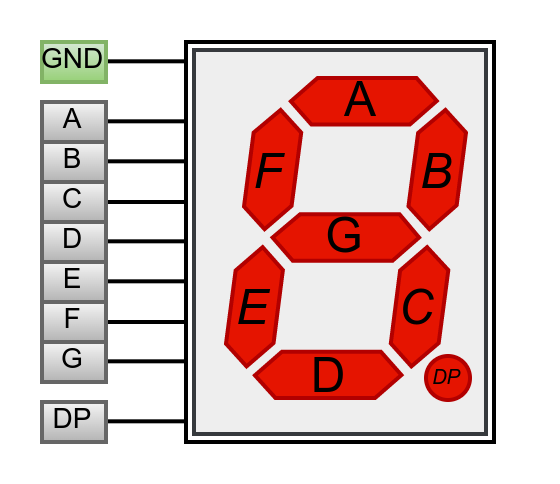
\includegraphics[width=0.39\textwidth]{7SEGMENT.png}
    \caption{Schema van het 7-segmentdisplay met een ``dp'' ($decimal$ $point$) ingang.}
    \label{fig:39110}
\end{figure}
\pagebreak
\subsection{Flip-flop's}
Een flip-flop is een geheugenelement dat in de elektronica wordt toegepast. Deze ``flip-flop'' wordt ook wel een ``bistabiele multivibrator'' genoemd. 
Elke soort flip-flop bestaat uit een bepaalde soort latch met één klokingang. Het input signaal voor de latch zal alleen doorgevoerd worden zodra de flank van de klokingang actief HOOG staat \cite{Flowers1983}. 
In dit verslag wordt er gewerkt met twee soorten flip-flop's, namelijk:
\begin{itemize}
    \item De D-flip-flop, wordt ook wel ``data-flip-flop'' genoemd, is een flip-flop dat een data-ingang D en een klokingang heeft;
    \item De J-K-flip-flop, is vernoemd naar ``Jack-Kilby-flip-flop''. Het is een flip-flop dat een klokingang en twee data-ingangen J en K bevat.
\end{itemize}
Zie hieronder de waarheidstabellen van de D-flip-flop en de J-K-flip-flop:
\begin{figure}[h]
    \begin{minipage}{.5\textwidth}
\begin{displaymath}
    \begin{array}{|c||c|c|c|}
    D & Q & \overline{Q} & Comments\\
    \hline 
    1 & 1 & 0 & SET \\
    0 & 0 & 1 & RESET
  \end{array}
    \end{displaymath}
\end{minipage}
\begin{minipage}{.5\textwidth}
\begin{displaymath}
    \begin{array}{|c|c||c|c|c|}
    J & K & Q & \overline{Q} & Comments\\
    \hline 
    0 & 0 & Q_{0} & \overline{Q_{0}} & No\ change\\
    0 & 1 & 0 & 1 & RESET\\
    1 & 0 & 1 & 0 & SET\\
    1 & 1 & \overline{Q_{0}} & Q_{0} & TOGGLE 
  \end{array}
    \end{displaymath}
\end{minipage}
\end{figure}
\\ 
Flip-flop klok signalen kunnen een positieve of een negatieve flank (edge) hebben. Dit houdt in dat de klokpuls pas wordt doorgevoerd aan het begin (positive edge) of einde (negative edge) van een puls. 
Positive edge klokpulsen worden aangegeven met een pijl omhoog en negative edge klokpulsen worden aangegeven met een pijl omlaag. 
Daarnaast kunnen flip-flop's worden toegepast in veel applicaties zoals in schuifregisters, frequentiedelers, dataopslag, tellers en nog veel meer. 
\begin{figure}[h]
    \centering
    \begin{minipage}{.5\textwidth}
      \centering
      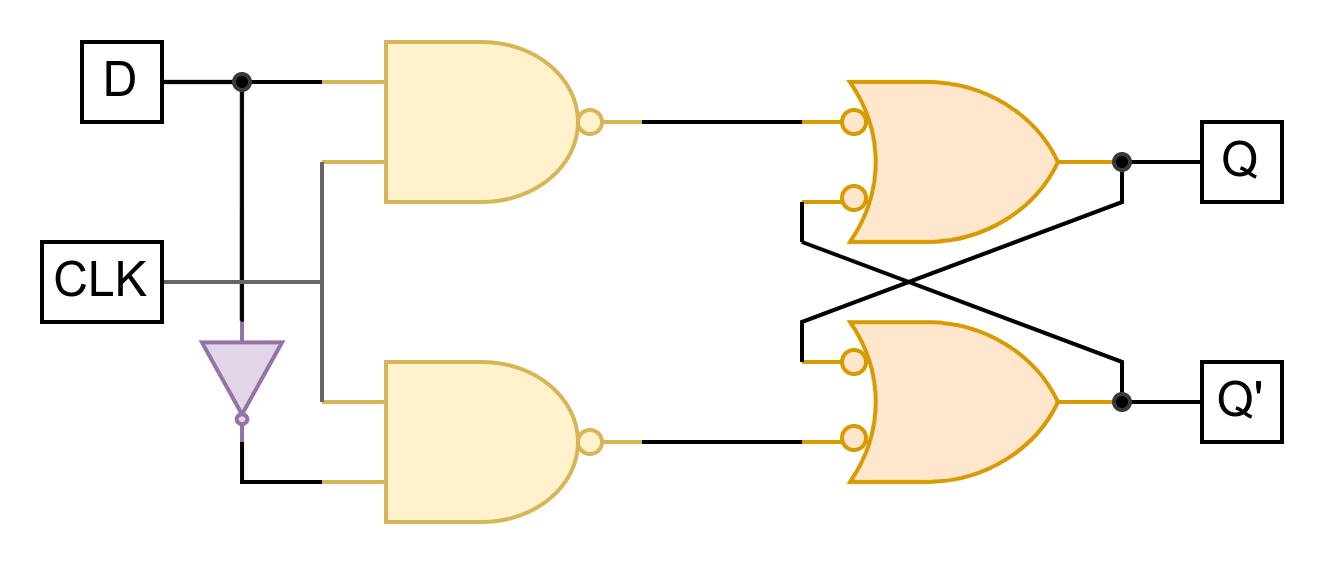
\includegraphics[width=1\linewidth]{dflip.png}
      \caption{Logische schakeling van de D-flip-flop.}
      \label{fig:dflipflop}
    \end{minipage}%
    \begin{minipage}{.5\textwidth}
      \centering
      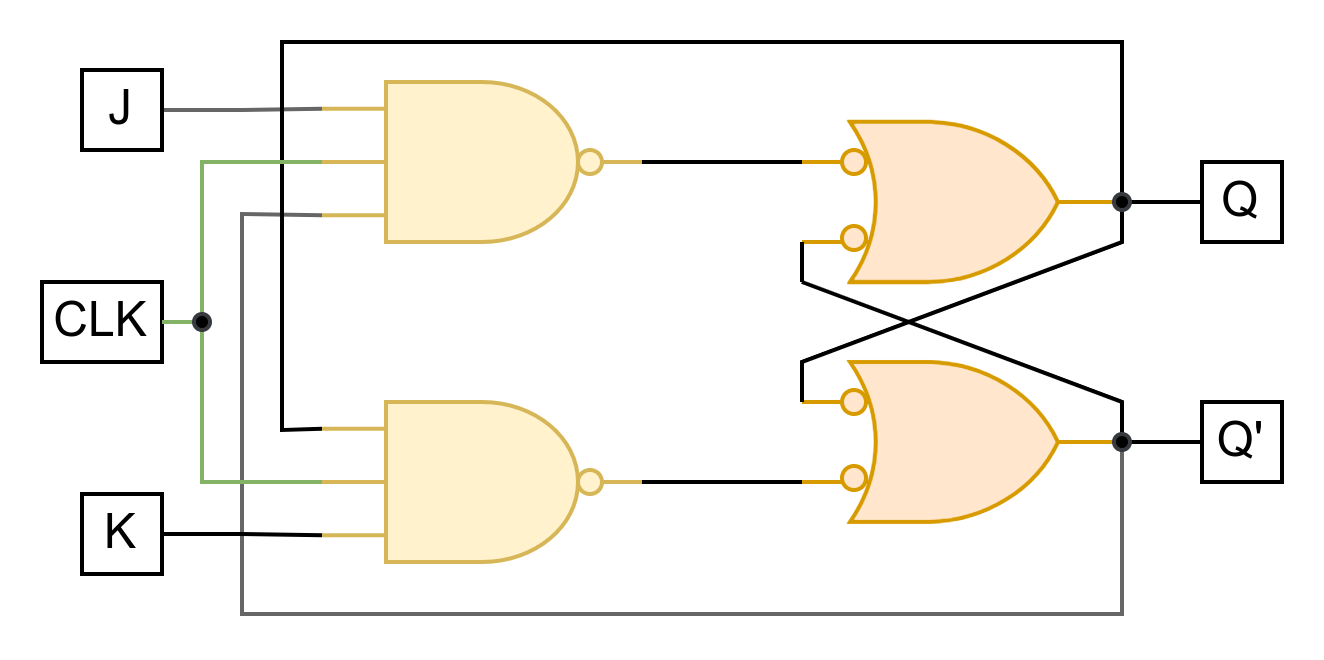
\includegraphics[width=1\linewidth]{jkflip.png}
      \caption{Logische schakeling van de J-K-flip-flop.}
      \label{fig:tessat2}
    \end{minipage}
    \end{figure}
\pagebreak
\subsection{Het 3910 digiboard: versie 2}
De ``Type 3910 DIGI BOARD 2'' is gefabriceerd door \textit{hps SystemTechnik} en is bedoeld als een universele trainingsbord om studenten te laten leren omgaan met logische schakelingen en poorten in de digitale techniek \cite{hps-systemtechnik}. 
Dit digiboard bevat de volgende ingebouwde componenten: \cite{hps-systemtechnik_ds_DIGI}
\begin{enumerate}
    \item 2 input keyboards with 4 pairs of keys (L/H) each;
    \item Clock generator with divider, TTL level, crystal-controlled;
    \item DC signal source 0...5 V/ 10 mA;
    \item Hexadecimal/dual coding switch (double);
    \item LED display, divided into 3 groups with the colors red, yellow, green;
    \item HIGH/LOW, for tapping HIGH, LOW states;
    \item 7-segment display (2-digit), with decoder: dual/7-segment;
    \item Adapter (2 mm jacks/SUB-D socket), for adapting 2 mm jacks to SUB-D connector (25-pin), pins 1...13 and 18 assigned;
    \item 8 AND gates, with pull-up Resistors, one gate is disconnectable;
    \item 6 OR gates, with pull-down Resistors, one gate is disconnectable;
    \item 3 AND/OR combi-gates;
    \item 1-bit comparator;
    \item 4-bit comparator;
    \item 4 J-K-flipflops, can also be used as RS flipflops;
    \item 4 D-flipflops;
    \item 2 adders (4-bit), with input and output carry;
    \item Monoflop, settable times: 0.1s; 1s; 5s;
    \item Multiplexer, 4 channels;
    \item Demultiplexer, 4 channels;
    \item Shift register (4-bit), parallel and serial operation possible, bidirectional;
    \item ALU, for conducting 16 arithmetic and 16 logical computing operations with 4-bit dual numbers;
    \item Binary counter (4-bit), up/down counter;
    \item 2 inverters with open collector (pull-up resistors can be connected);
    \item 2 Schmitt triggers, inverting;
    \item Units complements for negating a 4-bit binary number;
    \item Antivalence and equivalence gates;
    \item RAM 8x4, static RAM, 8 addresses, 4 bits data width;
    \item EEPROM 8x4, storage time without power supply approx. 1 hour;
    \item AD / DA converter (4-bit);
    \item Two slots for expanding a circuit with additional plug-in modules.
\end{enumerate}
Zie de afbeelding hieronder voor de representatie van het digiboard:
\begin{figure}[h]
    \centering
    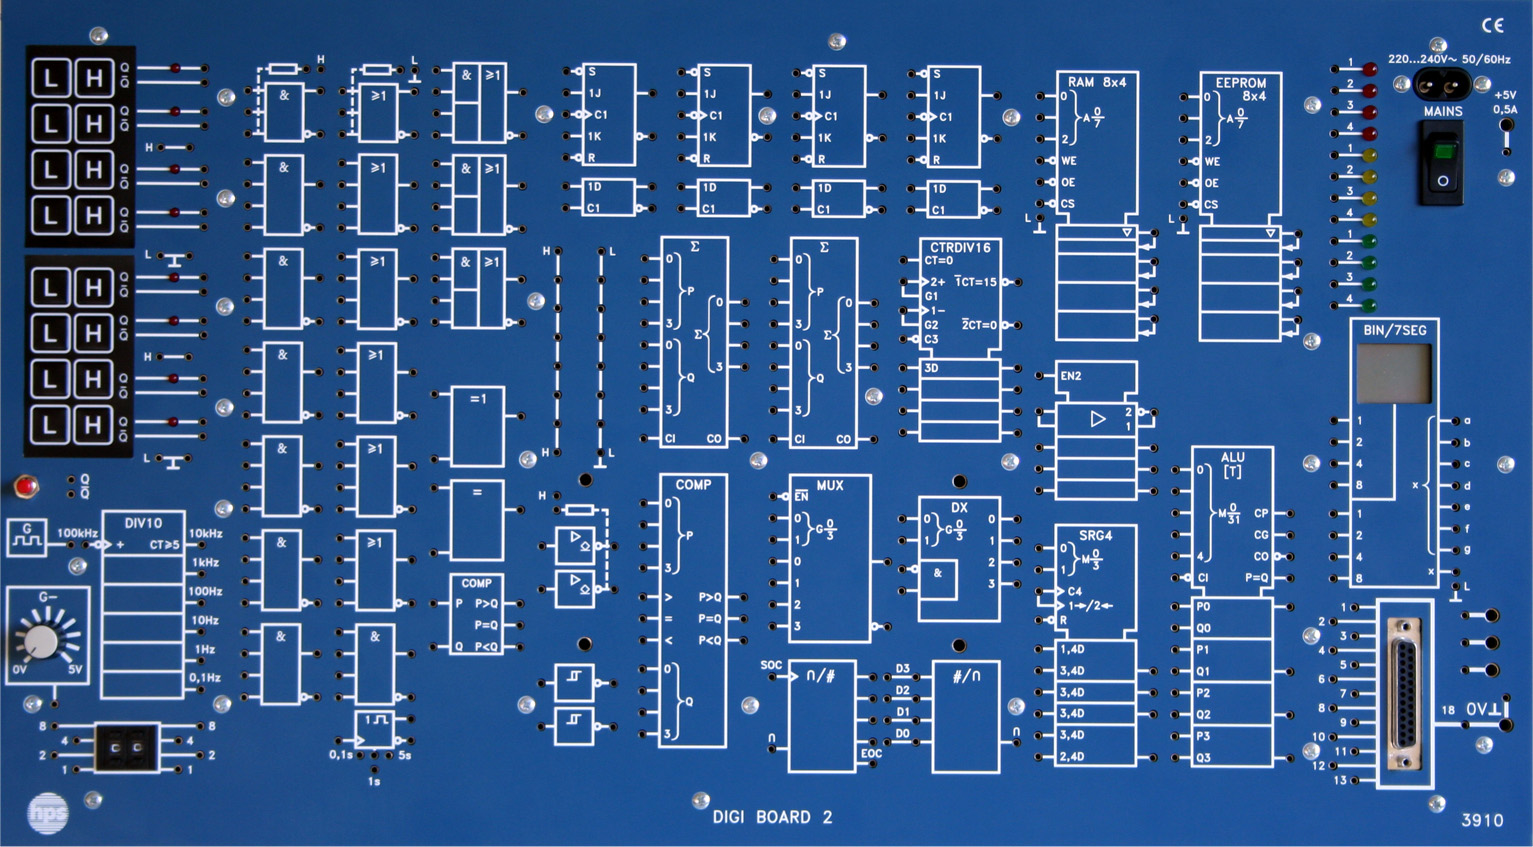
\includegraphics[width=0.8\textwidth]{3910.jpg}
    \caption{Foto van de ``Type 3910 DIGI BOARD 2''.}
    \label{fig:3910}
\end{figure}
\pagebreak
\section{Methode en aanpak}
Om dit practicum op een juiste manier uit te voeren is de volgende methodiek toegepast:\\
1. De voorbereiding voor het practicum:
\begin{itemize}
  \item De practicum benodigdhedenlijst (zie: H\ref{practicumbenodigdheden}) bekijken en de benodigdheden verzamelen en klaarzetten voor gebruik;
  \item Het theoretische kader (zie: H\ref{Theoretisch kader}) van dit verslag even goed doornemen zodat je weet hoe bepaalde materialen en de theorie in elkaar zit;
  \item De vragen van het practicum alvast bekijken en vervolgens zoeken naar mogelijke antwoorden zodat je dat (mogelijk) in ieder geval al klaar hebt staan. 
\end{itemize}
2. Het uitvoeren van het practicum:
\begin{itemize}
    \item Ga rustig door de vragen heen en noteer je antwoorden, als je iets niet weet kun je het altijd nog op internet zoeken of bij de bijbehorende docent een vraag stellen;
    \item Maak foto's van de logische schakelingen die je hebt gebouwd tijdens het practicum. Dit zodat je later in je mogelijke verslag kunt bewijzen dat je er ook echt was en alles werkend hebt gekregen;
    \item Ruim alle geleende spullen van school, zoals het digiboard, IC-board en snoeren weer netjes terug in het lab. Bewaar je antwoorden en gemaakte foto's op een juiste manier, zodat je later netjes een verslag kunt schrijven. 
\end{itemize}
3. Het schrijven van het verslag:
\begin{itemize}
    \item Maak een document voor dit practicum en geef een gepaste naam aan je document;
    \item Zorg ervoor dat je in ieder geval een: voorblad, inhoudsopgave, inleiding, probleemstelling, theoretisch kader, methode, resultaten, conclusie en bronvermeldingen in het verslag hebt staan;
    \item Op het voorblad zet je de naam van het verslag, je eigen naam (met evt. studentennummer erbij) en datum;
    \item In je inleiding schrijf je kort een introductie over het practicum zelf en geef je het algemene doel van het verslag aan;
    \item In het theoretisch kader geef je uitleg over de toegepaste theorie tijdens het practicum, hierbij zijn bronnen erg belangrijk;
    \item In de methode geef je uitleg over hoe je alles hebt aangepakt en uitgewerkt hebt, zodat de lezer het practicum mogelijk zelf zou kunnen uitvoeren;
    \item De resultaten/antwoorden splits je op in secties net zoals de vragen zijn gesteld in het practicum bestand. Deze resultaten werk je netjes uit en zet je de gemaakte foto's en schema's in de bijbehorende vraag;
    \item In de conclusie geef je antwoord op je probleemstelling en gestelde doelen aan de hand van je resultaten en bespreek ook de belangrijke bevindingen die je had tijdens het practicum;
    \item Tenslotte moet je ook bronvermeldingen hebben. Hierin staan alle gebruikte bronnen, zoals datasheets, artikelen, verslagen, literatuur en overige online bronnen. Dit zodat de lezer kan checken waar je bepaalde informatie vandaan hebt gehaald en mogelijk meer kan lezen over de gebruikte informatie.
\end{itemize}
\pagebreak
\section{Combinatorische logische functie: MUX}
In de eerste opdracht zijn de volgende deelvragen onderzocht en beantwoord over de multiplexer:
\begin{enumerate}
    \item Stel de waarheidstabel op voor een 4-bit multiplexer;
    \item Herleid vanuit de opgestelde waarheidstabel de bijbehorende logische uitdrukking; 
    \item Teken de logische schakeling die deze uitdrukking representeert;
    \item Bouw de schakeling op het digiboard;
    \item Controleer de werking van de logische schakeling. 
\end{enumerate}
\begin{figure}[h]
    \centering
    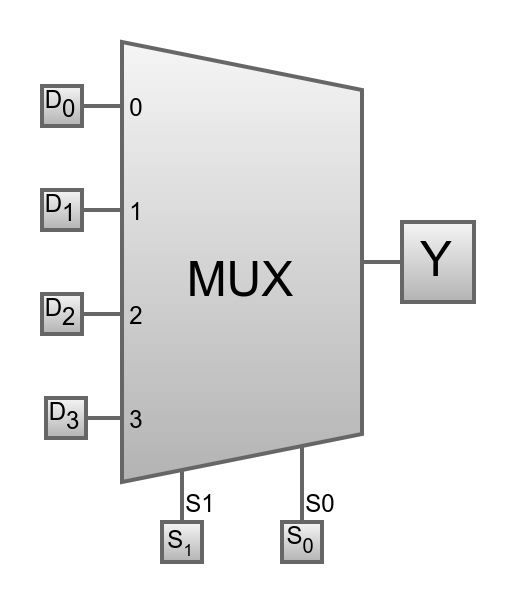
\includegraphics[width=0.5\textwidth]{mux3.png}
    \caption{Een 4-bit multiplexer (afgekort MUX).}
    \label{fig:mux43}
\end{figure}
\pagebreak
\subsection{Stel de waarheidstabel op voor de 4-bit multiplexer}
Zie de opgestelde waarheidstabel van de 4-bit multiplexer (figuur \ref{fig:mux43}):
\begin{displaymath}
    \begin{array}{|c|c||c|}
    S_{1} & S_{0} & Input\ Selected \\
    \hline 
    0 & 0 & D_{0} \\
    0 & 1 & D_{1} \\
    1 & 0 & D_{2} \\
    1 & 1 & D_{3}
    \end{array}
    \end{displaymath}
\subsection{Herleid vanuit de opgestelde waarheidstabel de bijbehorende logische uitdrukking}
De bijbehorende logische uitdrukking: $D_0 \cdot \overline{S_1} \cdot \overline{S_0} + D_1 \cdot \overline{S_1} \cdot S_0 + D_2 \cdot S_1 \cdot \overline{S_0} + D_3 \cdot S_1 \cdot S_0$.
\subsection{Teken de logische schakeling die deze uitdrukking representeert}
\begin{figure}[h]
    \centering
    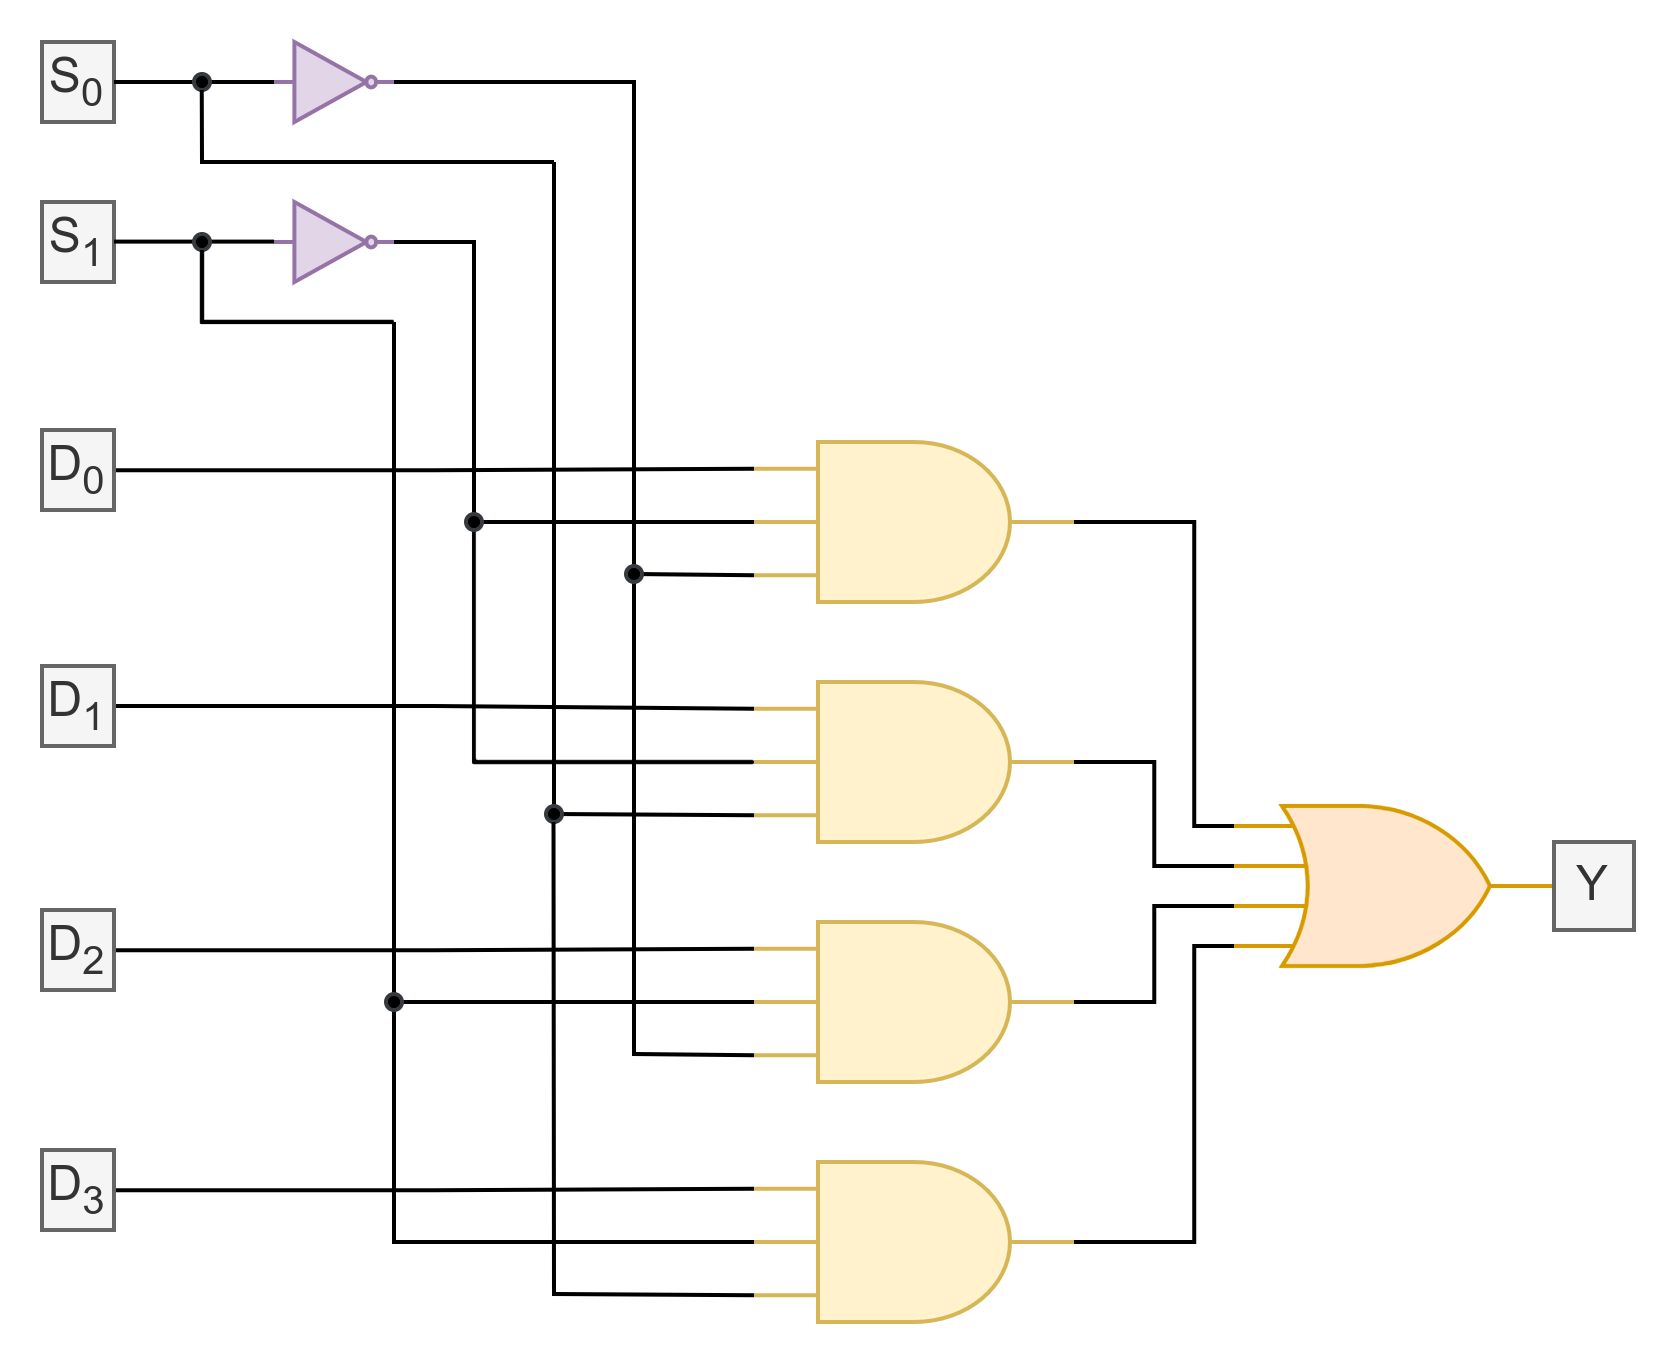
\includegraphics[width=0.8\textwidth]{mux2.png}
    \caption{Ontwerp van de logische schakeling van de 4-bit multiplexer. Deze MUX heeft twee select pennen en vier data pennen.}
    \label{fig:mux2}
\end{figure}
\pagebreak
\subsection{Bouw de schakeling op het digiboard}
\begin{figure}[h]
    \centering
    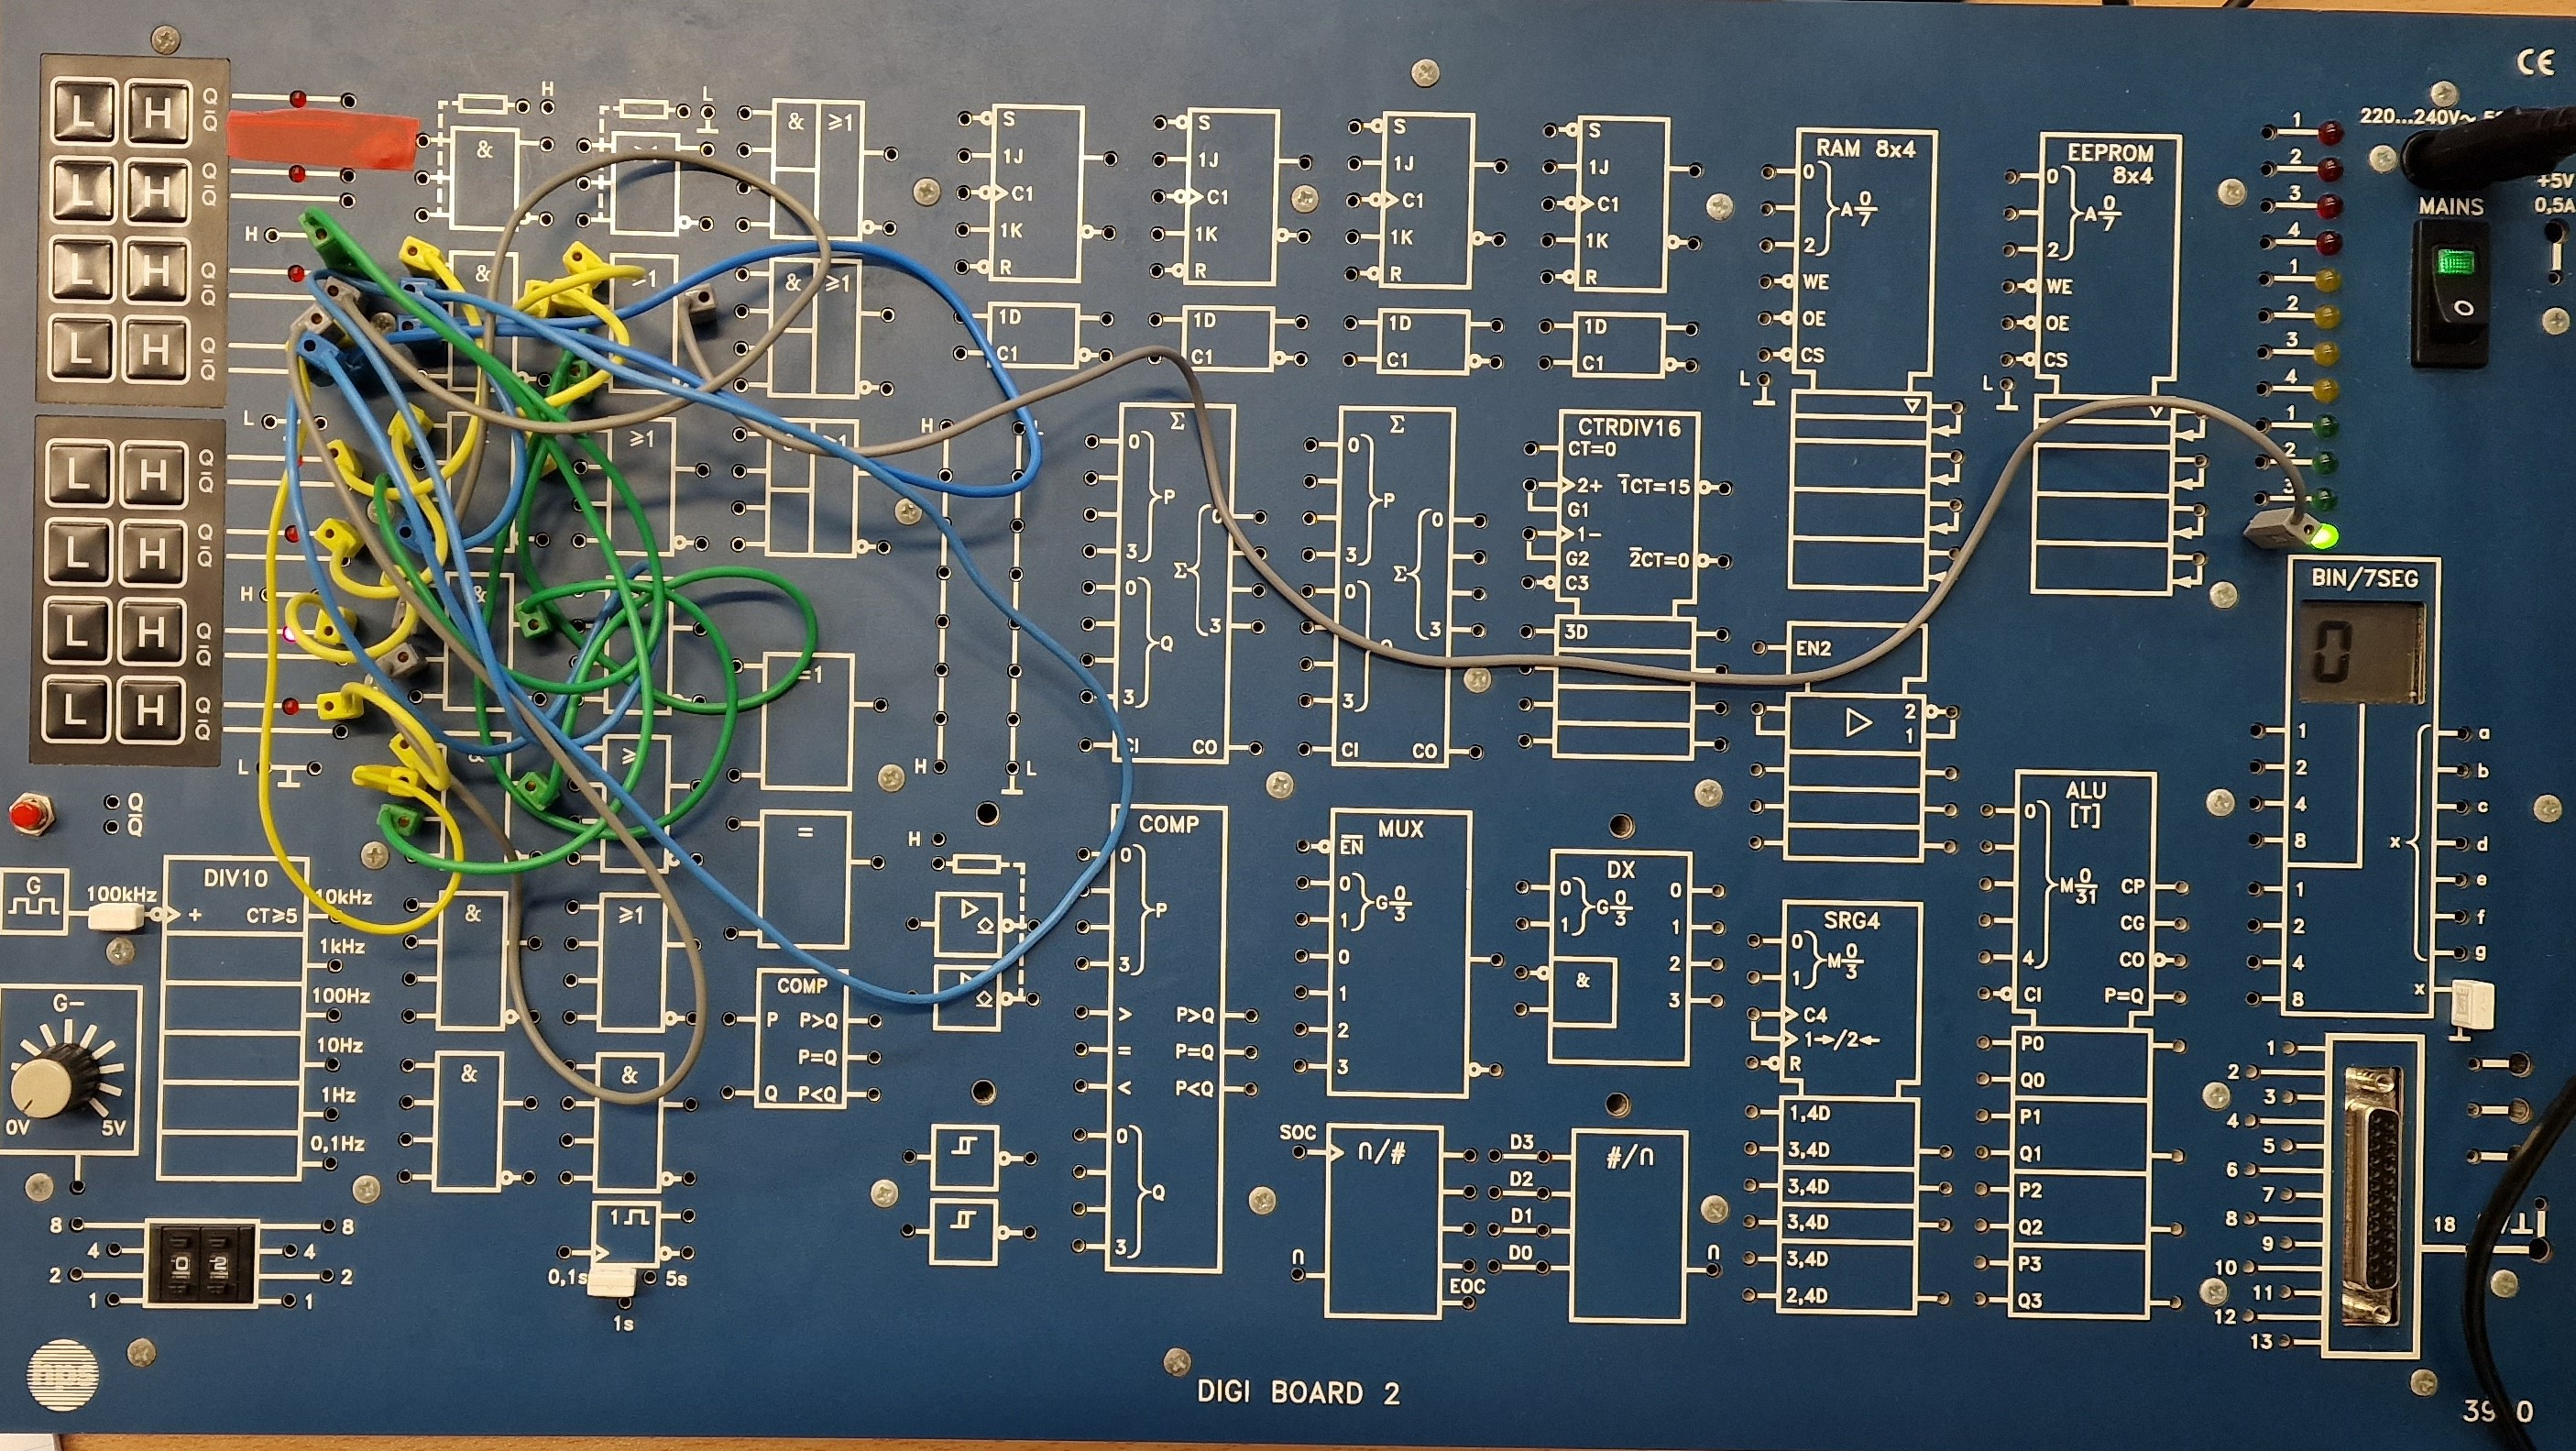
\includegraphics[width=0.8\textwidth]{mux.jpg}
    \caption{Foto van de ontworpen logische schakeling van de multiplexer dat gebouwd is op het digiboard.}
    \label{fig:muxsxie}
\end{figure}
\subsection{Controleer de werking van de logische schakeling}
Tijdens het practicum is het ontworpen logische schakeling gebouwd op het digiboard en werkte de multiplexer succesvol. 
Zie de resultaten hieronder: 
\begin{itemize}
    \item De data-uitgang $y$ is alleen gelijk aan $D_0$ wanneer $S_1$ = 0 en $S_0$ = 0;
    \item De data-uitgang $y$ is alleen gelijk aan $D_1$ wanneer $S_1$ = 0 en $S_0$ = 1;
    \item De data-uitgang $y$ is alleen gelijk aan $D_2$ wanneer $S_1$ = 1 en $S_0$ = 0;
    \item De data-uitgang $y$ is alleen gelijk aan $D_3$ wanneer $S_1$ = 1 en $S_0$ = 1.
\end{itemize}
Dit komt overeen met de eerder opgestelde waarheidstabel en de logische uitdrukking: $D_0 \cdot \overline{S_1} \cdot \overline{S_0} + D_1 \cdot \overline{S_1} \cdot S_0 + D_2 \cdot S_1 \cdot \overline{S_0} + D_3 \cdot S_1 \cdot S_0$.
\pagebreak
\section{Combinatorische logische functie: BCD-encoder}
In de tweede opdracht zijn de volgende deelvragen onderzocht en beantwoord over de BCD-encoder:
\begin{enumerate}
    \item Stel een BCD-tabel op voor decimale getallen 0 t/m 9;
    \item Herleid vanuit deze opgestelde tabel de bijbehorende logische uitdrukking;
    \item Teken de logische schakeling die deze uitdrukking representeert;
    \item Bouw de schakeling op het digiboard;
    \item Controleer de werking van de logische schakeling door de BCD-uitgangen aan te sluiten op de BIN/7SEG decoder. 
\end{enumerate}
\pagebreak
\subsection{Stel een BCD-tabel op voor decimale getallen 0 t/m 9}
\begin{displaymath}
    \begin{array}{|c||c|c|c|c|}
    Decimaal & \overbrace{A|B|C|D}^{Binary-Coded-Decimal} \\
    \hline 
    0 & 0 | 0 | 0 | 0 \\
    1 & 0 | 0 | 0 | 1 \\
    2 & 0 | 0 | 1 | 0 \\
    3 & 0 | 0 | 1 | 1 \\
    4 & 0 | 1 | 0 | 0 \\
    5 & 0 | 1 | 0 | 1 \\
    6 & 0 | 1 | 1 | 0 \\
    7 & 0 | 1 | 1 | 1 \\
    8 & 1 | 0 | 0 | 0 \\
    9 & 1 | 0 | 0 | 1
    \end{array}
    \end{displaymath}
\subsection{Herleid vanuit deze opgestelde tabel de bijbehorende logische uitdrukking}
De bijbehorende logische uitdrukkingen voor de BCD-encoder:
\begin{itemize}
    \item $A\ (X_3)=A\ \overline{B}\ \overline{C}\ \overline{D} + A\ \overline{B}\ \overline{C}\ D$;
    \item $B\ (X_2)=\overline{A}\ B\ \overline{C}\ \overline{D} + \overline{A}\ B\ \overline{C}\ D + \overline{A}\ B\ C\ \overline{D} + \overline{A}\ B\ C\ D$;
    \item $C\ (X_1)=\overline{A}\ \overline{B}\ C\ \overline{D} + \overline{A}\ \overline{B}\ C\ D + \overline{A}\ B\ C\ \overline{D} + \overline{A}\ B\ C\ D$;
    \item $D\ (X_0)=\overline{A}\ \overline{B}\ \overline{C}\ D + \overline{A}\ \overline{B}\ C\ D + \overline{A}\ B\ \overline{C}\ D+ \overline{A}\ B\ C\ D + A\ \overline{B}\ \overline{C}\ D$.
\end{itemize}
\pagebreak
\subsection{Teken de logische schakeling die deze uitdrukking representeert}
Zie de ontworpen logische schakeling hieronder:
\begin{figure}[h]
    \centering
    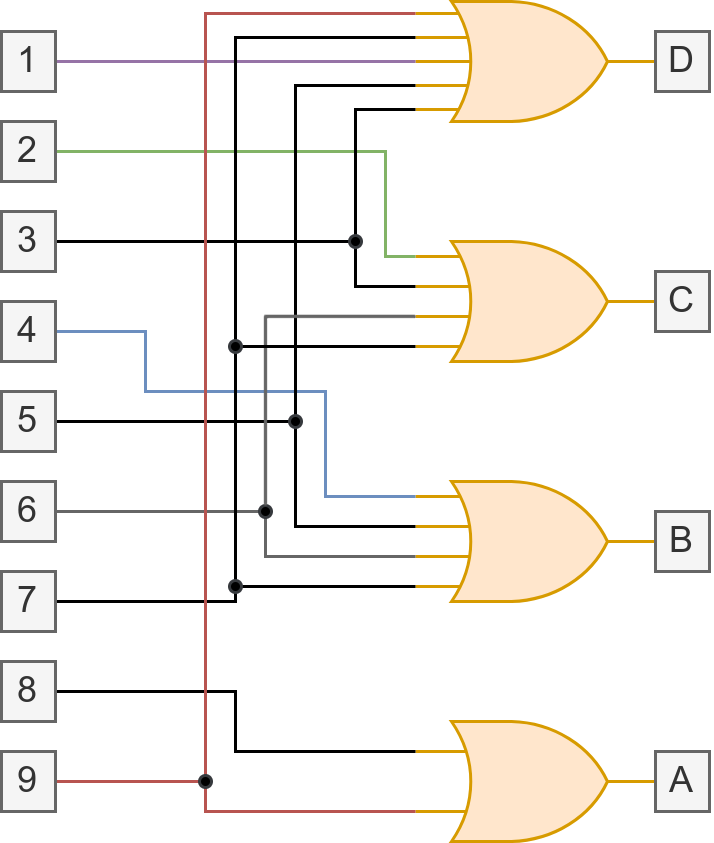
\includegraphics[width=0.8\textwidth]{bcd.png}
    \caption{Logische schakeling van de BCD-encoder. Het getal `0' is hierbij niet meegenomen, omdat bij dat getal er geen LED aangaat (binair: 0000).}
    \label{fig:bcd}
\end{figure}
\pagebreak
\subsection{Bouw de schakeling op het digiboard}
\begin{figure}[h]
    \centering
    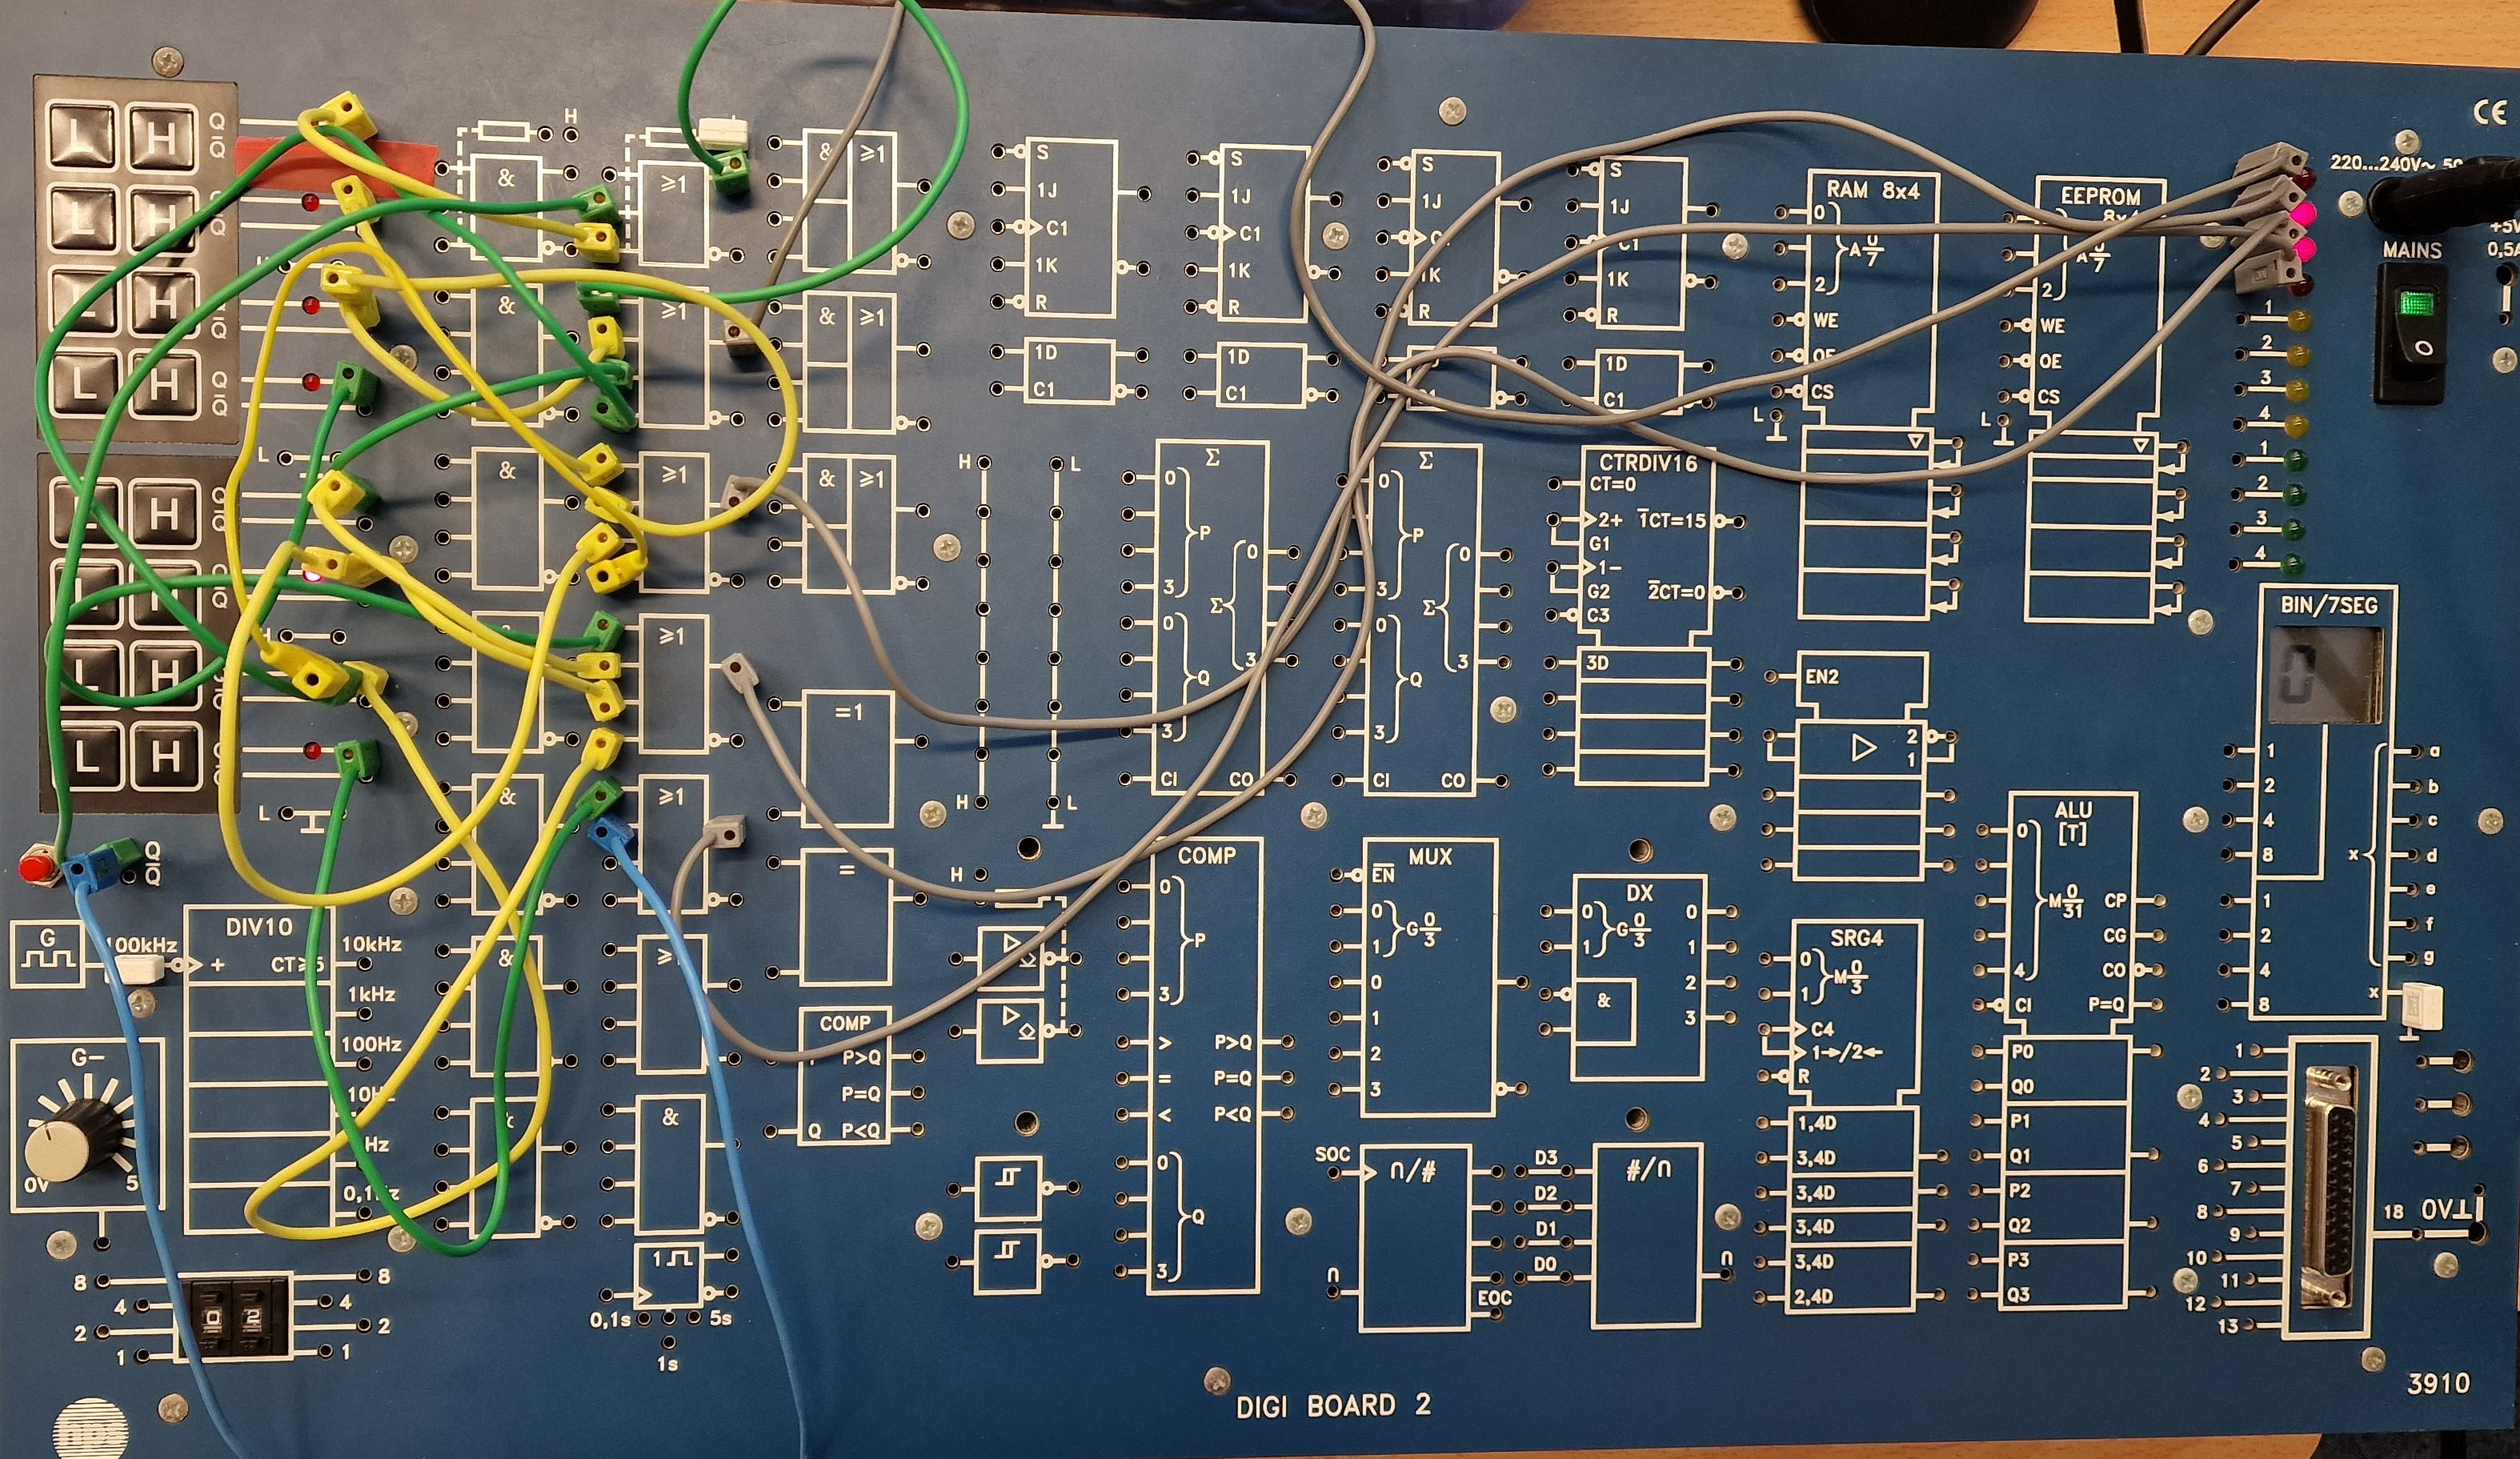
\includegraphics[width=0.7\textwidth]{bcdled.jpg}
    \caption{Foto van de gebouwde logische schakeling van de BCD-encoder.}
    \label{fig:bcdled}
\end{figure}
\subsection{Controleer de werking van de logische schakeling door de BCD-uitgangen aan te sluiten op de BIN/7SEG decoder}
Tijdens het practicum is de output aangesloten aan de BIN/7SEG decoder en werkt het allemaal zoals het zou moeten, zie de afbeelding hieronder:
\begin{figure}[h]
    \centering
    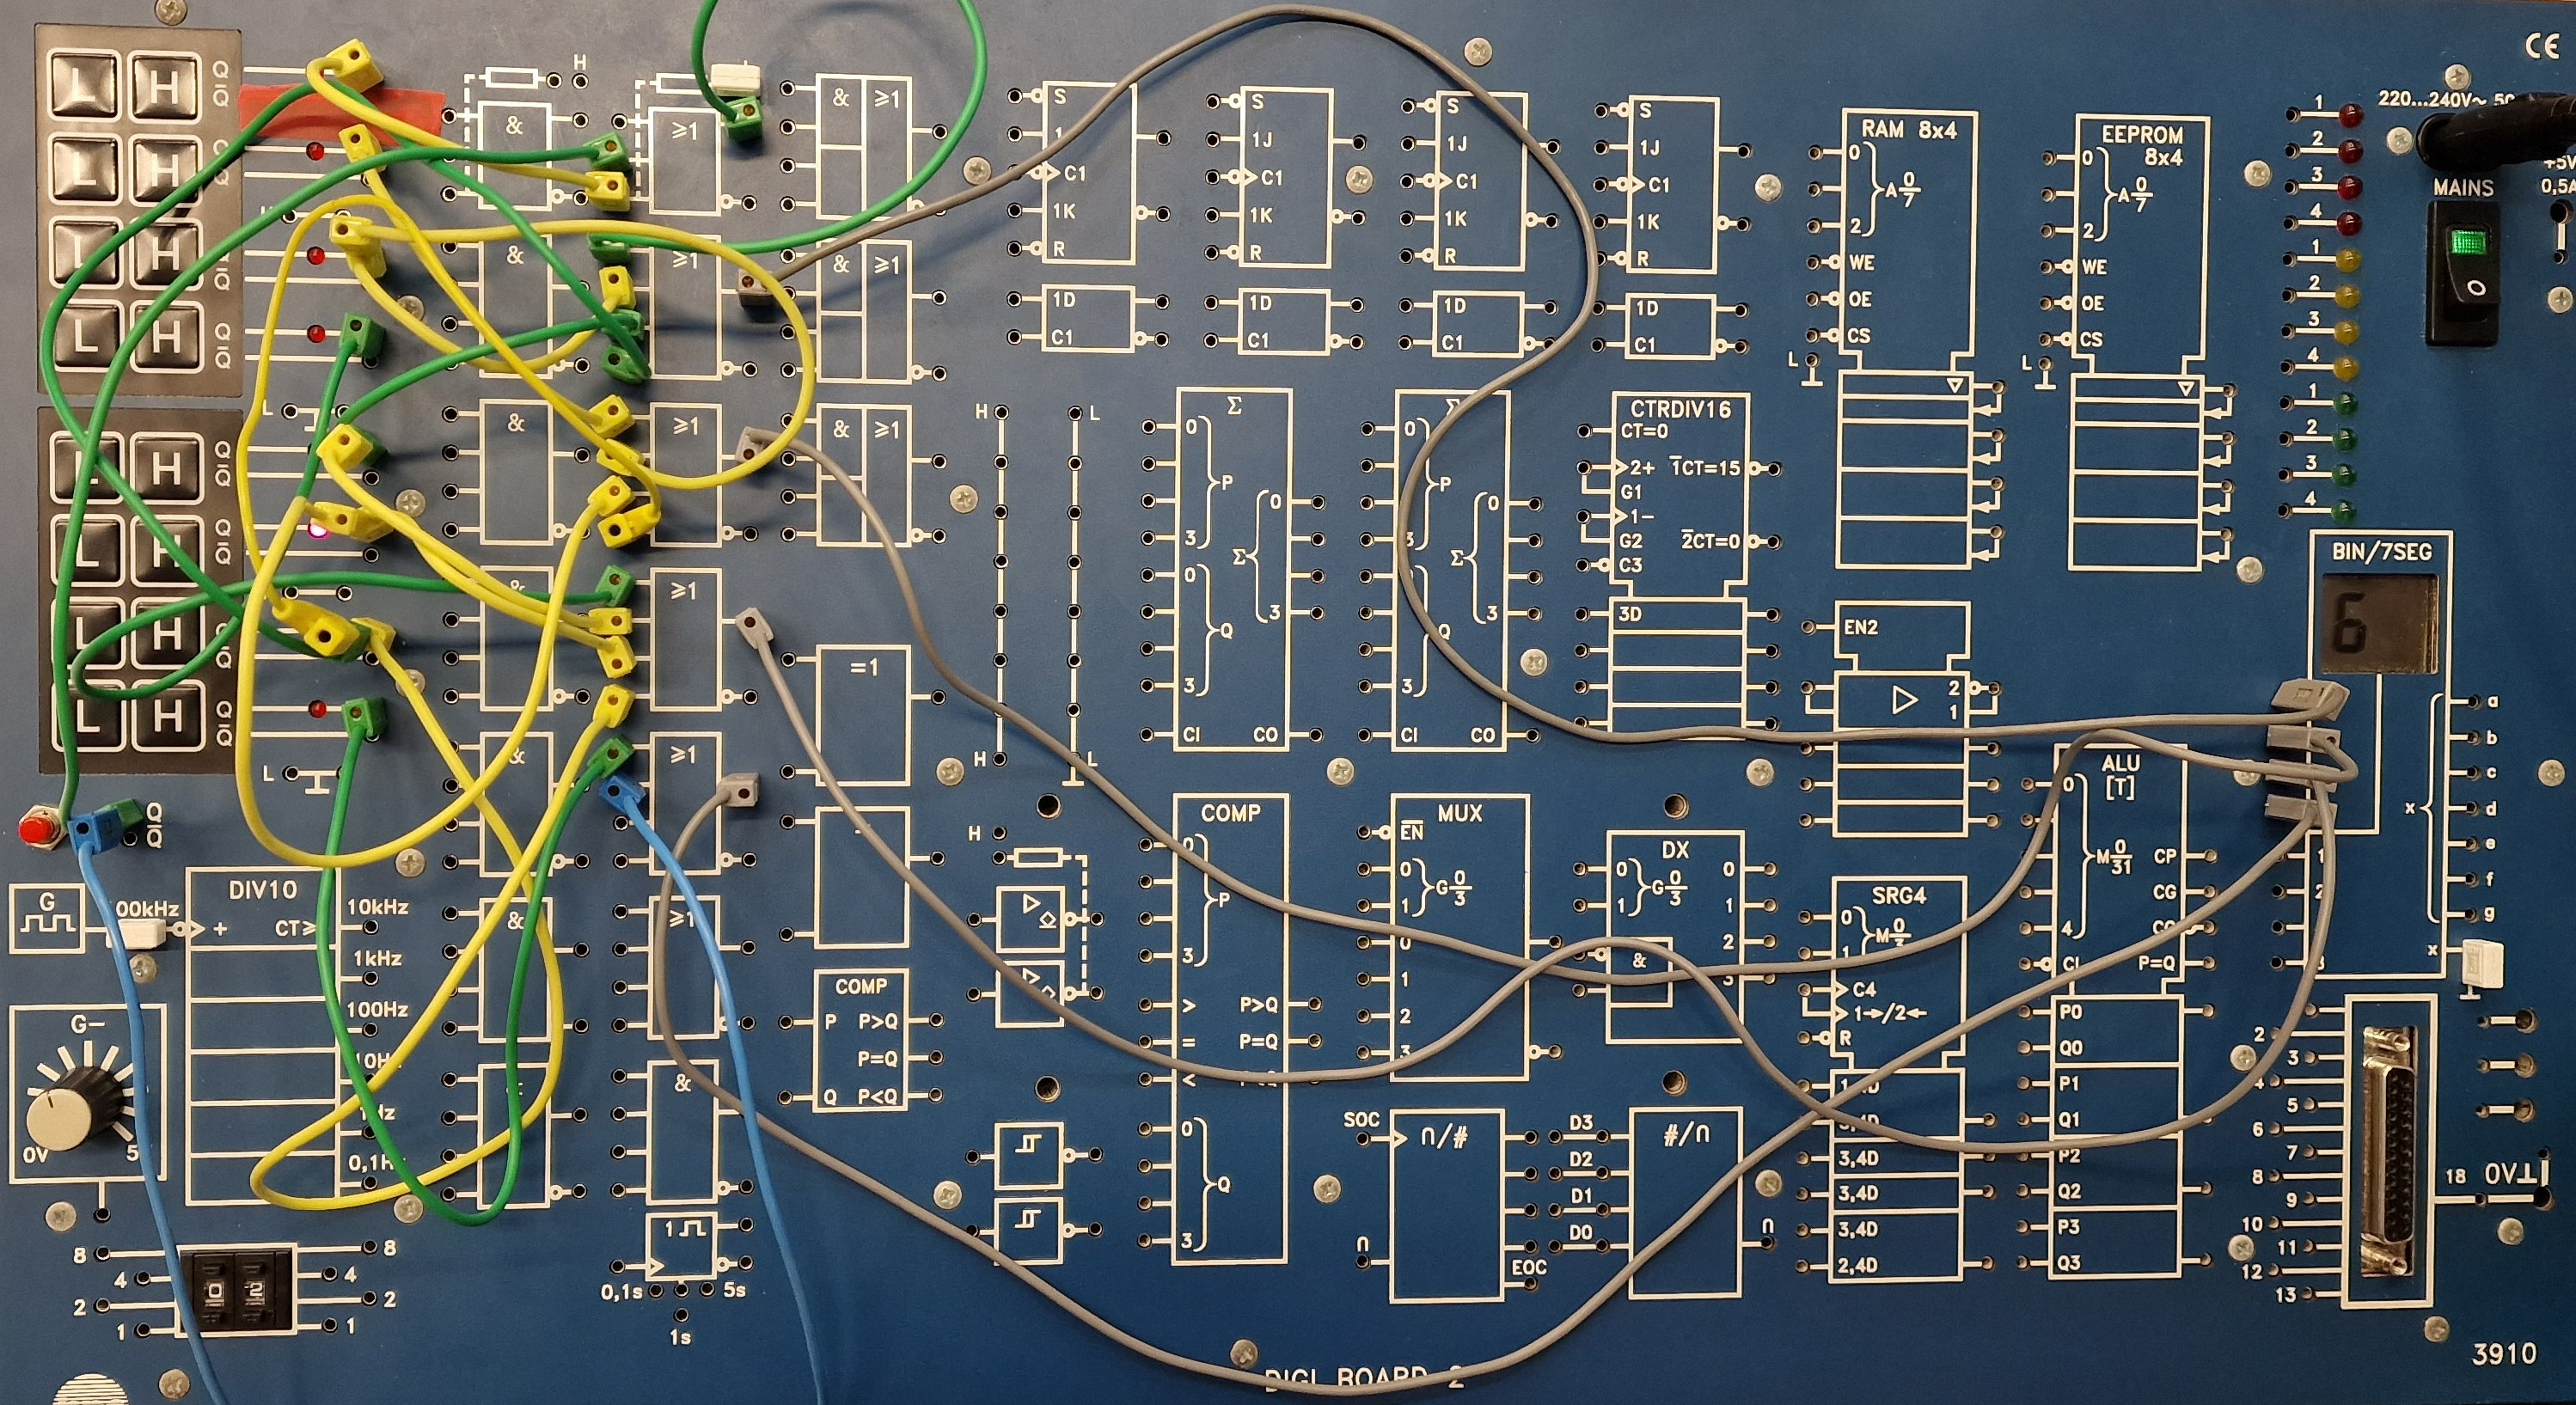
\includegraphics[width=0.7\textwidth]{bcd7.jpg}
    \caption{Foto van de gebouwde logische schakeling van de BCD-encoder waarbij de output is aangesloten aan een BIN/7SEG decoder.}
    \label{fig:bcd7}
\end{figure}
\pagebreak
\section{Teller (2N-toestanden)}
In de derde opdracht zijn de volgende deelvragen onderzocht en beantwoord over de teller met 2N-toestanden:
\begin{enumerate}
    \item Ontwerp met behulp van 4 J-K-flip-flops een teller met 2N toestanden;
    \item Stel aan de hand van het ontwerp, de bijbehorende toestandstabel op;
    \item Hoe wordt deze teller ook wel genoemd;
    \item Bouw deze schakeling op het digiboard;
    \item Sluit de uitgang van elke flip-flop aan op een LED;
    \item Sluit op de klokingang van de J-K-flip-flops een blokgolf met een frequentie van 1 Hz aan (gebruik hiervoor de DIV 10 generator die zich op het digiboard bevindt);
    \item Controleer of de schakeling alle toestanden doorloopt;
    \item Eigenschappen en tijdvolgordediagram.
\end{enumerate}
\pagebreak
\subsection{Ontwerp met behulp van 4 J-K-flip-flops een teller met 2N toestanden}
\begin{figure}[h]
    \centering
    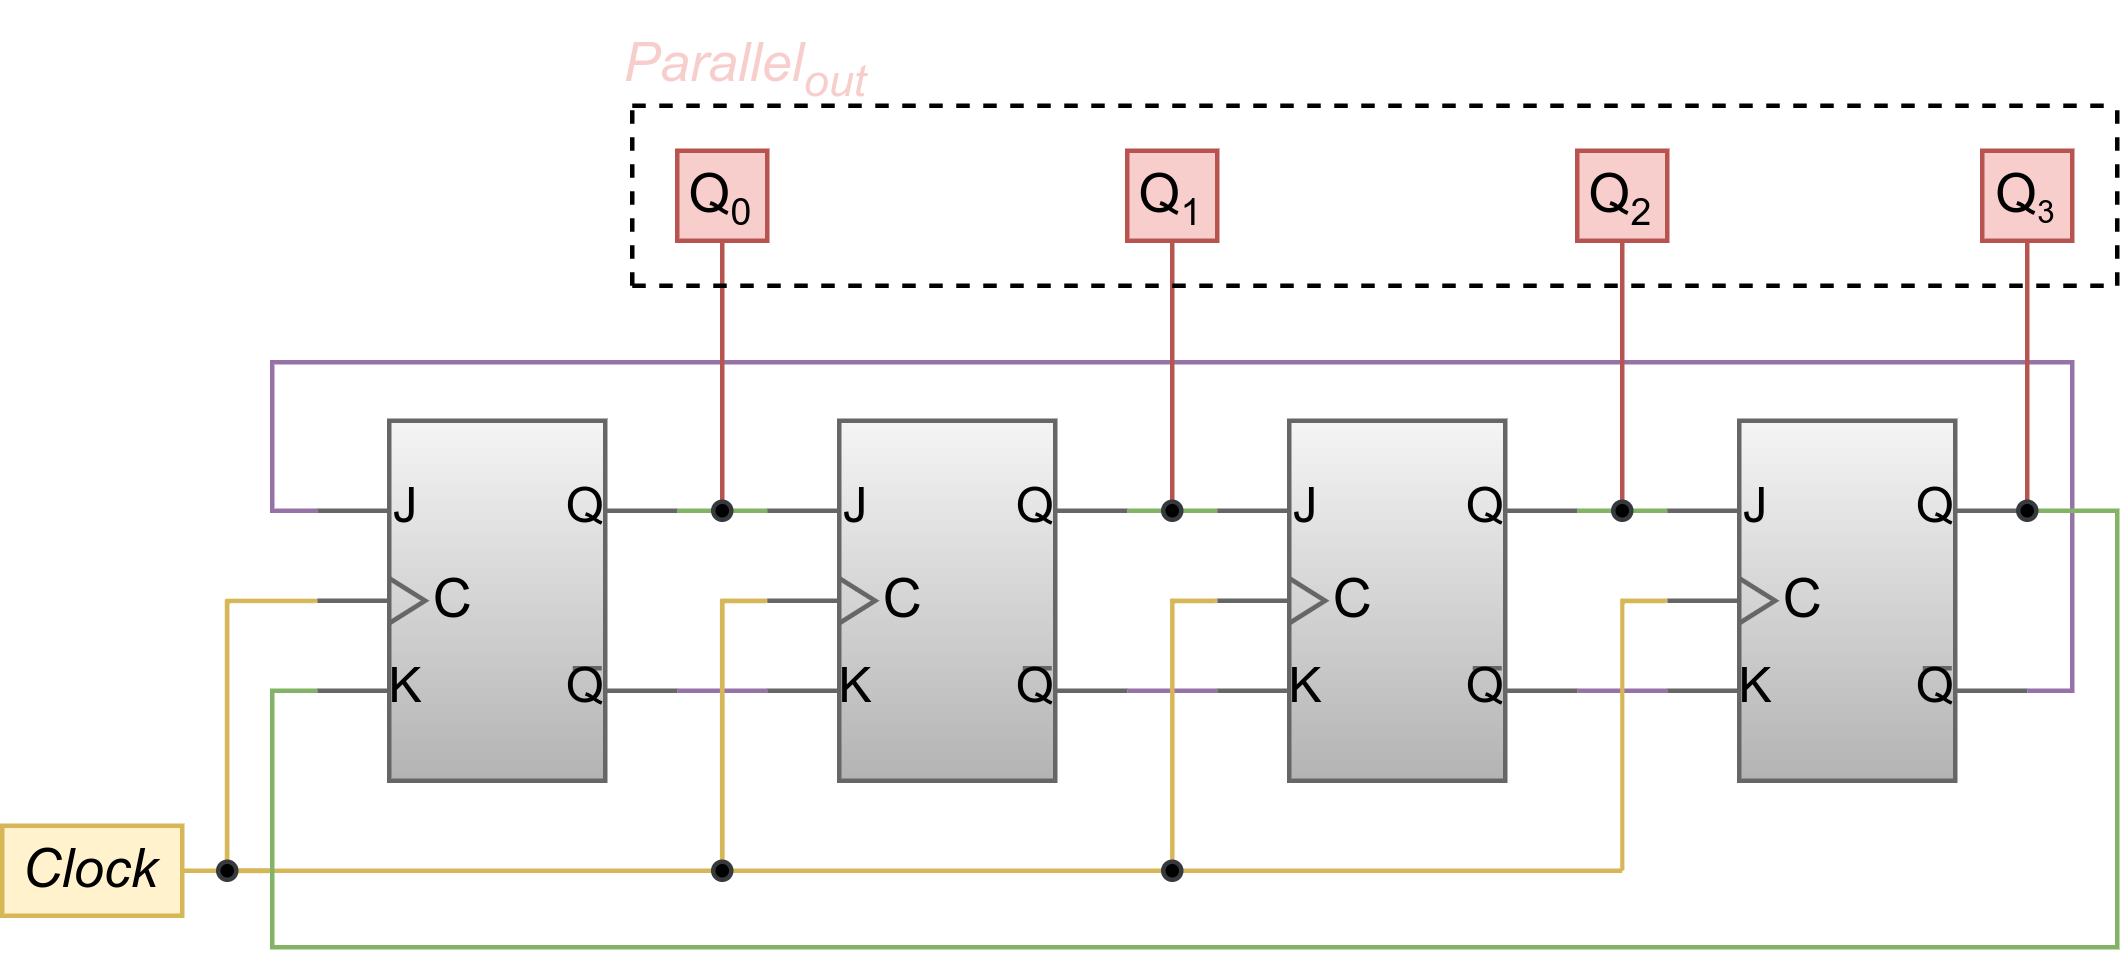
\includegraphics[width=0.8\textwidth]{john.png}
    \caption{Logische schakeling van de 2N Teller.}
    \label{fig:john}
\end{figure} 
\subsection{Stel aan de hand van het ontwerp, de bijbehorende toestandstabel op}
\label{lol2}
De Johnsonteller heeft 2N toestanden, dat betekent dat er maximaal acht mogelijke toestanden zijn (0 tot en met 7) \cite{1lol}. 
Zie hieronder de bijbehorende toestandstabel van de twisted ring counter (Johnsonteller):
\begin{table}[h]
    \centering
    \begin{tabular}{|lllll|}
    \hline
    \multicolumn{5}{|c|}{\textbf{Twisted ring counter}}                                                                                                 \\ \hline
    \multicolumn{1}{|l|}{\textbf{Toestand}} & \multicolumn{1}{l|}{\textbf{$Q_{0}$}} & \multicolumn{1}{l|}{\textbf{$Q_{1}$}} & \multicolumn{1}{l|}{\textbf{$Q_{2}$}} & \textbf{$Q_{3}$} \\ \hline
    \multicolumn{1}{|l|}{\textbf{0}} & \multicolumn{1}{l|}{0}          & \multicolumn{1}{l|}{0}          & \multicolumn{1}{l|}{0}          & 0          \\ \hline
    \multicolumn{1}{|l|}{\textbf{1}} & \multicolumn{1}{l|}{\textbf{1}} & \multicolumn{1}{l|}{0}          & \multicolumn{1}{l|}{0}          & 0          \\ \hline
    \multicolumn{1}{|l|}{\textbf{2}} & \multicolumn{1}{l|}{\textbf{1}} & \multicolumn{1}{l|}{\textbf{1}} & \multicolumn{1}{l|}{0}          & 0          \\ \hline
    \multicolumn{1}{|l|}{\textbf{3}} & \multicolumn{1}{l|}{\textbf{1}} & \multicolumn{1}{l|}{\textbf{1}} & \multicolumn{1}{l|}{\textbf{1}} & 0          \\ \hline
    \multicolumn{1}{|l|}{\textbf{4}}        & \multicolumn{1}{l|}{\textbf{1}}  & \multicolumn{1}{l|}{\textbf{1}}  & \multicolumn{1}{l|}{\textbf{1}}  & \textbf{1}  \\ \hline
    \multicolumn{1}{|l|}{\textbf{5}} & \multicolumn{1}{l|}{0}          & \multicolumn{1}{l|}{\textbf{1}} & \multicolumn{1}{l|}{\textbf{1}} & \textbf{1} \\ \hline
    \multicolumn{1}{|l|}{\textbf{6}} & \multicolumn{1}{l|}{0}          & \multicolumn{1}{l|}{0}          & \multicolumn{1}{l|}{\textbf{1}} & \textbf{1} \\ \hline
    \multicolumn{1}{|l|}{\textbf{7}} & \multicolumn{1}{l|}{0}          & \multicolumn{1}{l|}{0}          & \multicolumn{1}{l|}{0}          & \textbf{1} \\ \hline
    \multicolumn{1}{|l|}{\textbf{0}} & \multicolumn{1}{l|}{0}          & \multicolumn{1}{l|}{0}          & \multicolumn{1}{l|}{0}          & 0          \\ \hline
    \end{tabular}
    \end{table}
\pagebreak
\subsection{Hoe wordt deze teller ook wel genoemd}
Deze teller met 2N toestanden wordt ook wel een ``Johnson counter'' of ``Twisted ring counter'' genoemd. De `Q' output van de laatste J-K-flip-flop is verbonden aan K van de eerste J-K-flip-flop en hetzelfde principe geldt ook voor $\overline{Q}$ naar J. 
Dit is de reden waarom het een ``twisted'' ring counter wordt genoemd, maar ook omdat het een ring structuur heeft. Zie de afbeelding hieronder van de twisted ring counter:
\begin{figure}[h]
    \centering
    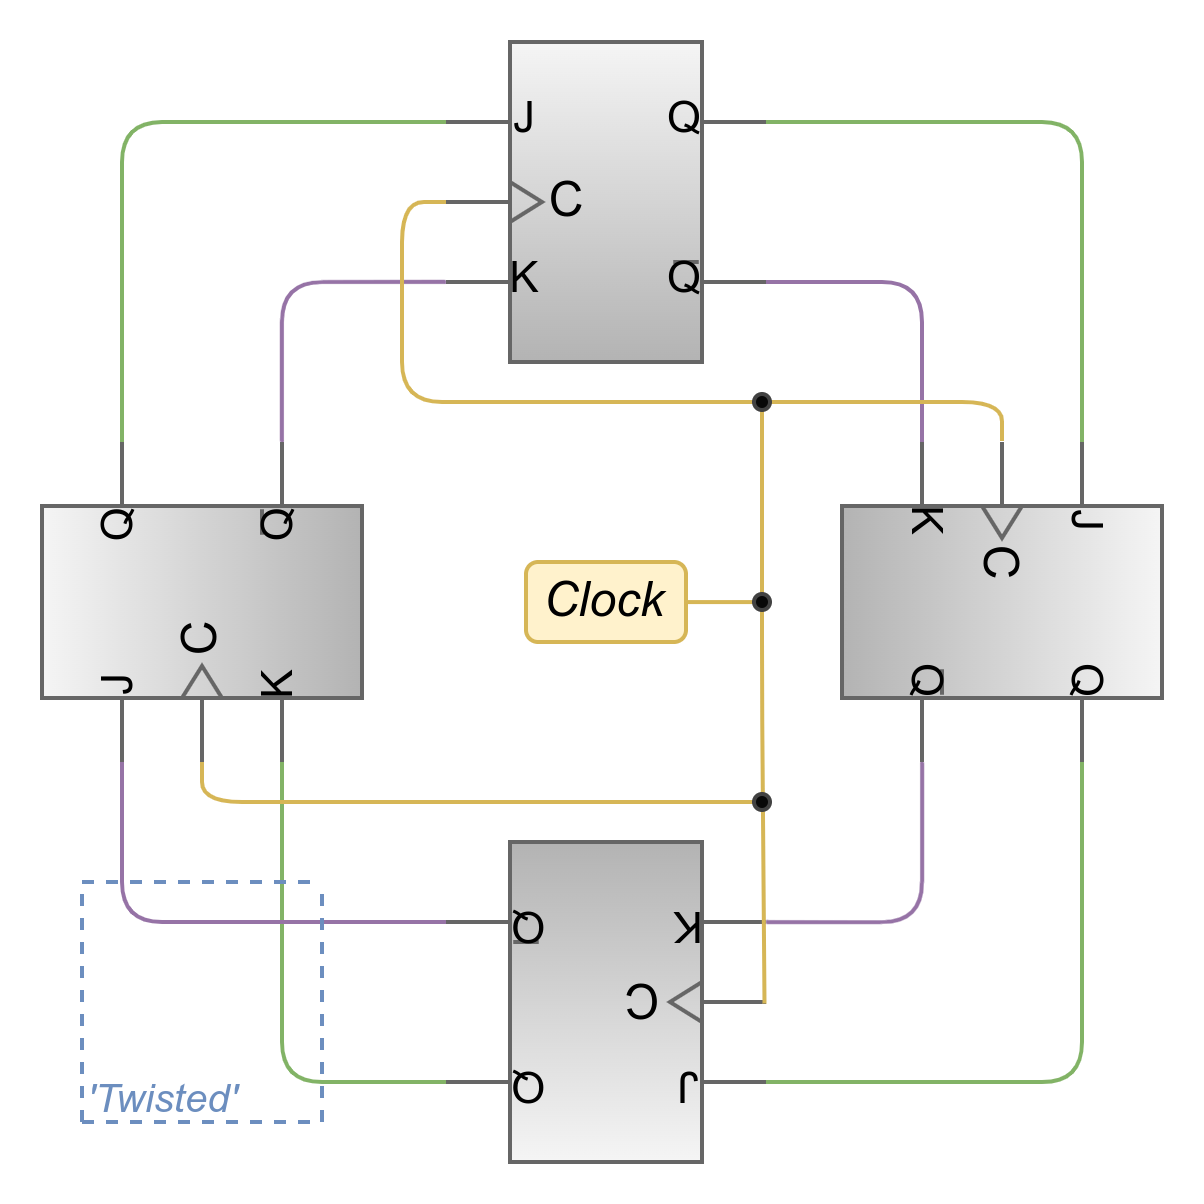
\includegraphics[width=0.8\textwidth]{johnring.png}
    \caption{Logische schakeling van twisted ring counter.}
    \label{fig:john2}
\end{figure}
\pagebreak 
\subsection{Bouw deze schakeling op het digiboard}
\begin{figure}[h]
    \centering
    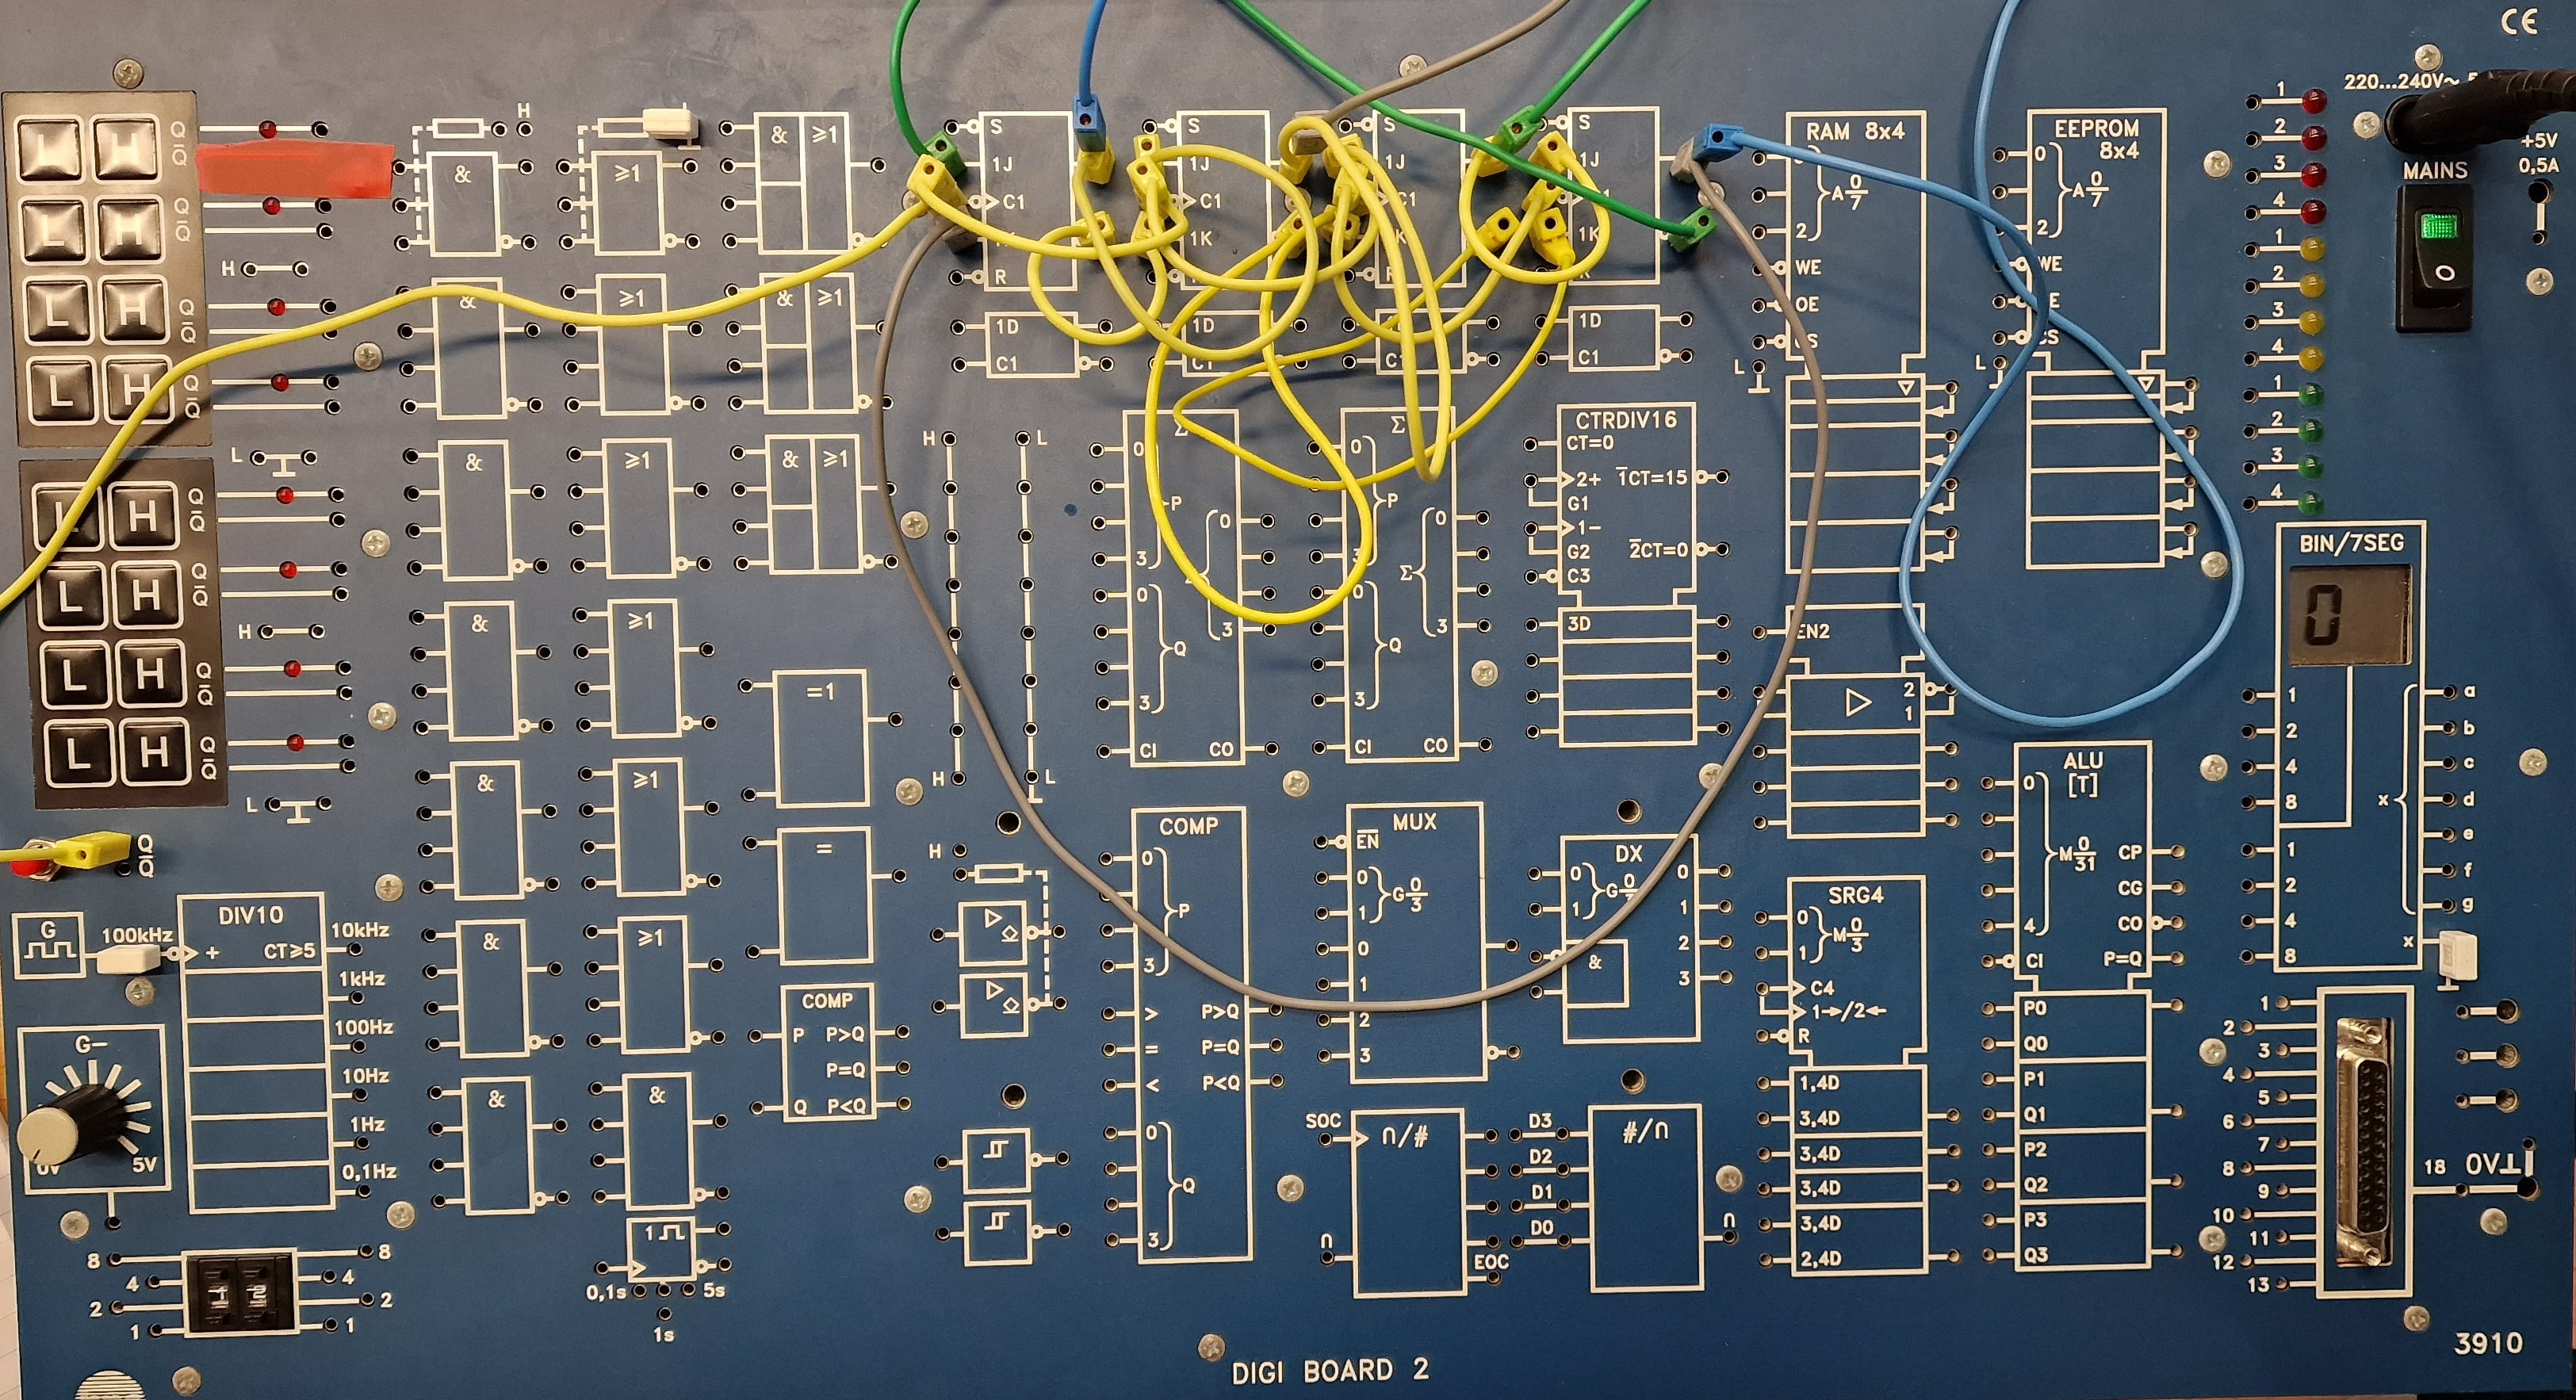
\includegraphics[width=0.7\textwidth]{1jc.jpg}
    \caption{Gebouwde logische schakeling van twisted ring counter.}
    \label{fig:john11}
\end{figure} 
\subsection{Sluit de uitgang van elke flip-flop aan op een LED}
\begin{figure}[h]
    \centering
    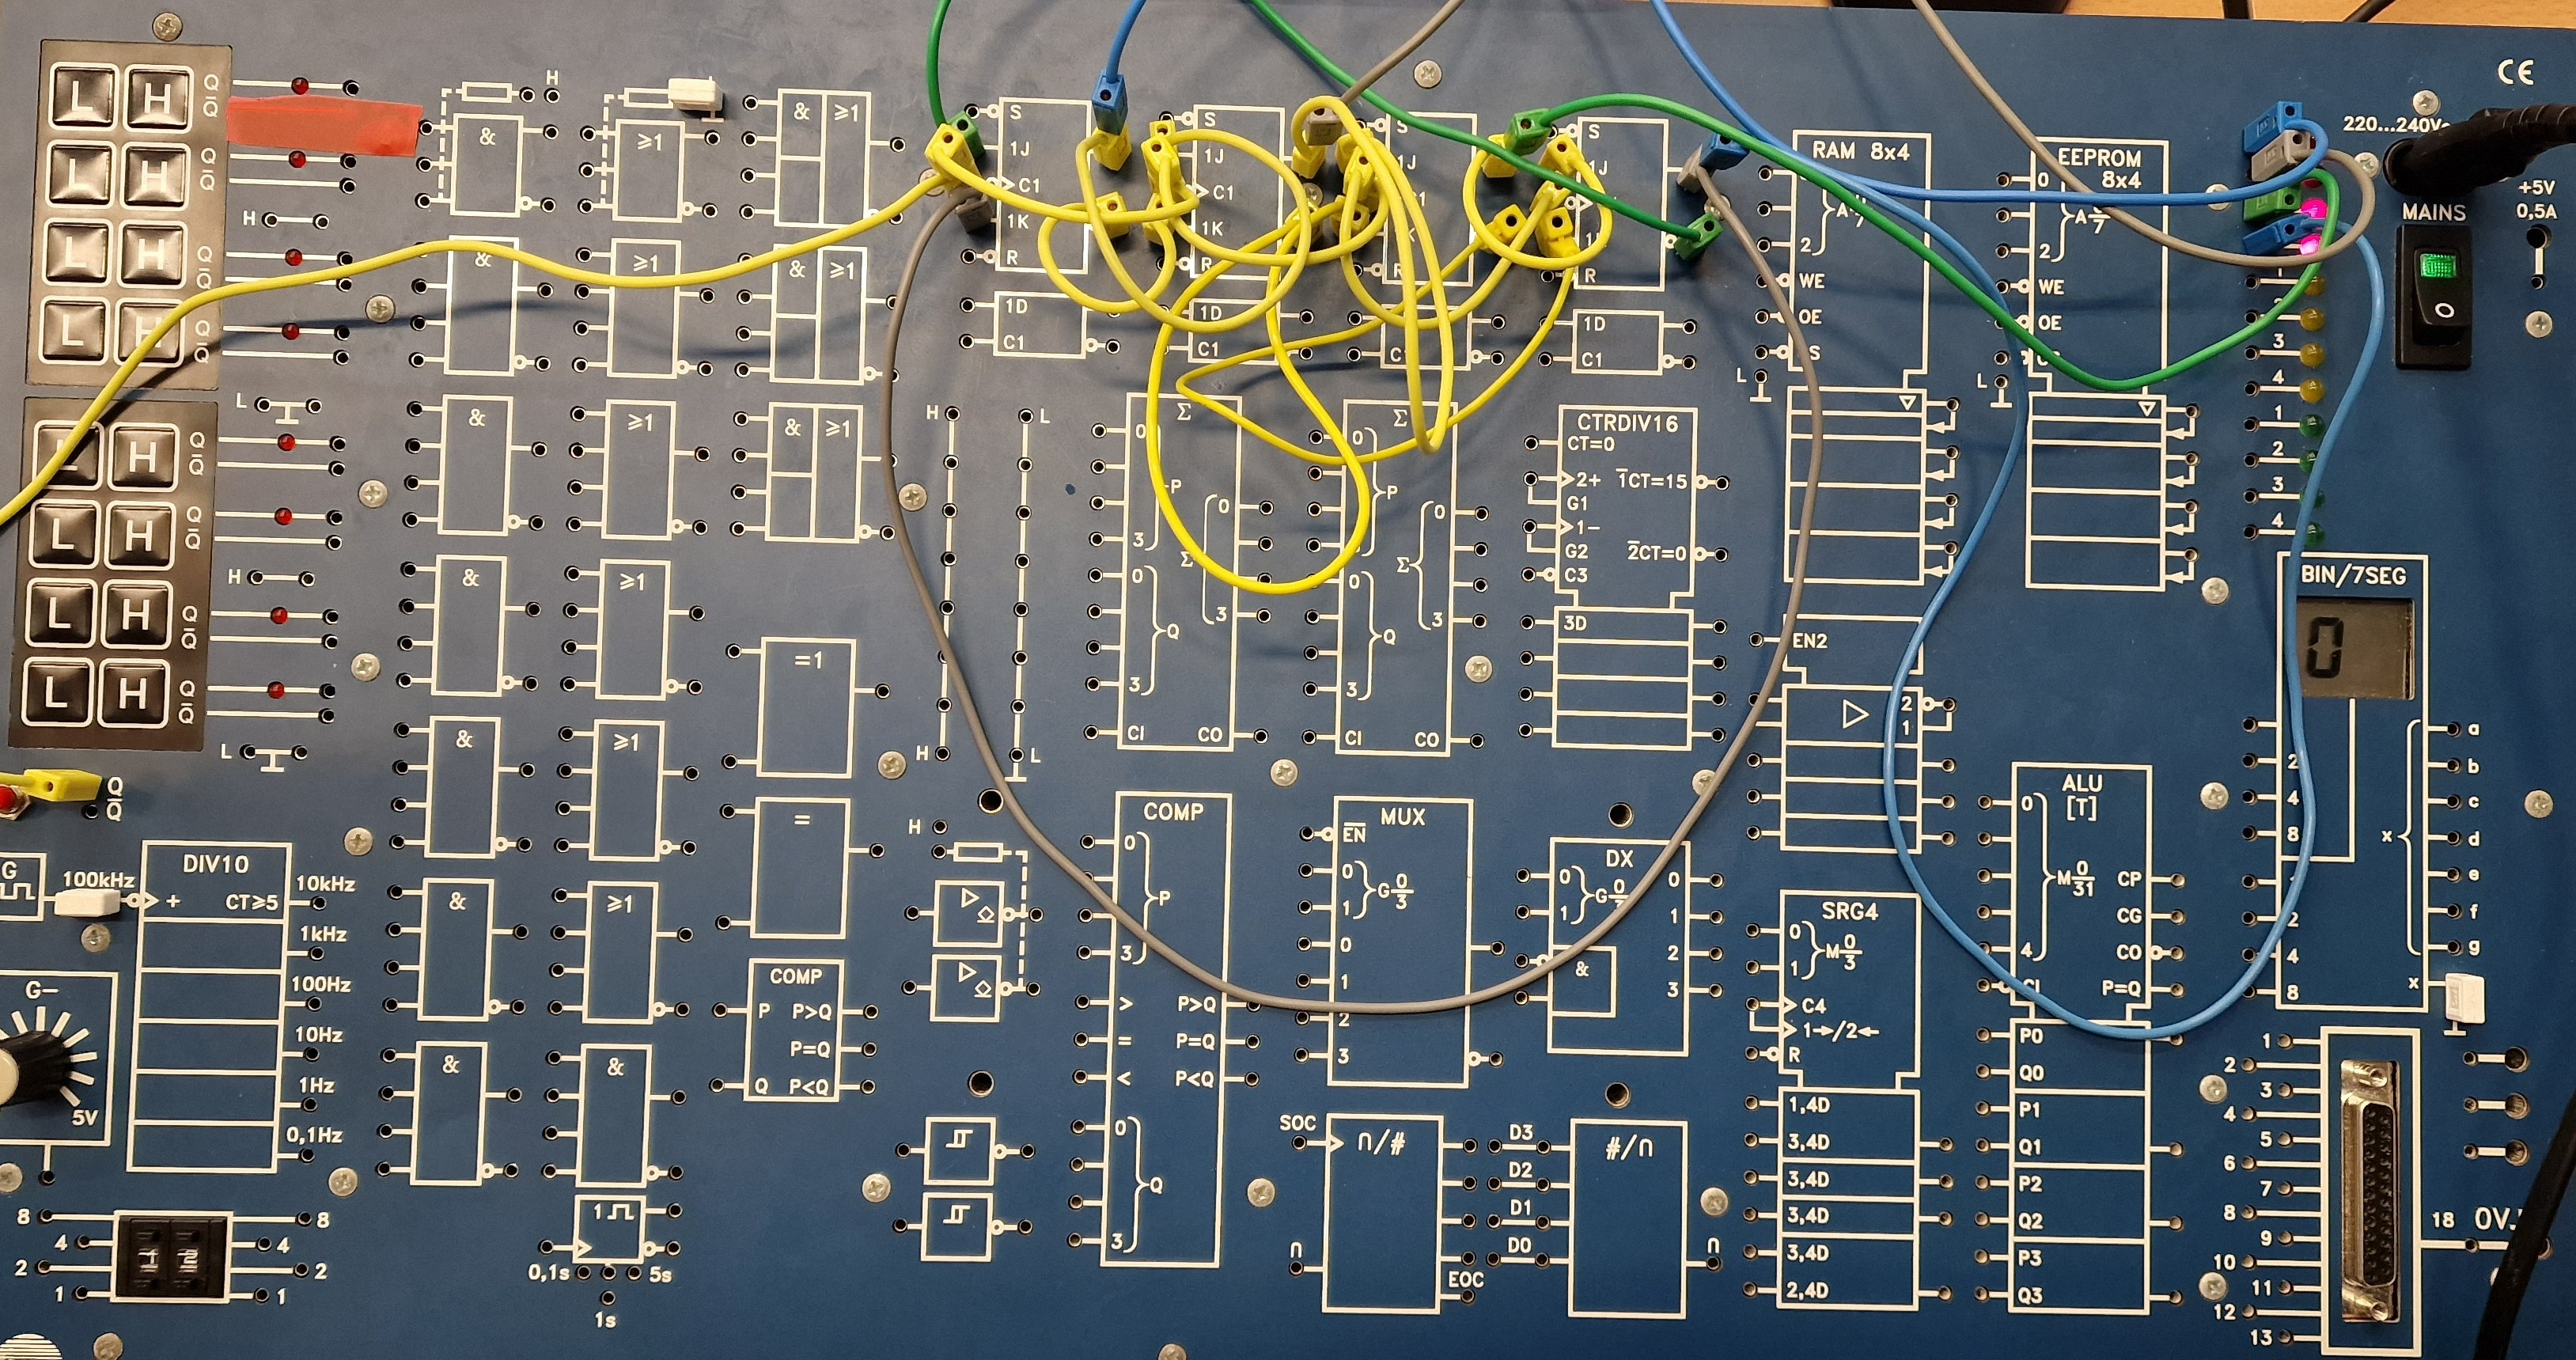
\includegraphics[width=0.7\textwidth]{1jc2.jpg}
    \caption{Gebouwde logische schakeling van twisted ring counter. De output snoeren zijn aangesloten aan LED's.}
    \label{fig:john112}
\end{figure} 
\pagebreak 
\subsection{Sluit op de klokingang van de J-K-flip-flops een blokgolf met een frequentie van 1 Hz aan}
\begin{figure}[h]
    \centering
    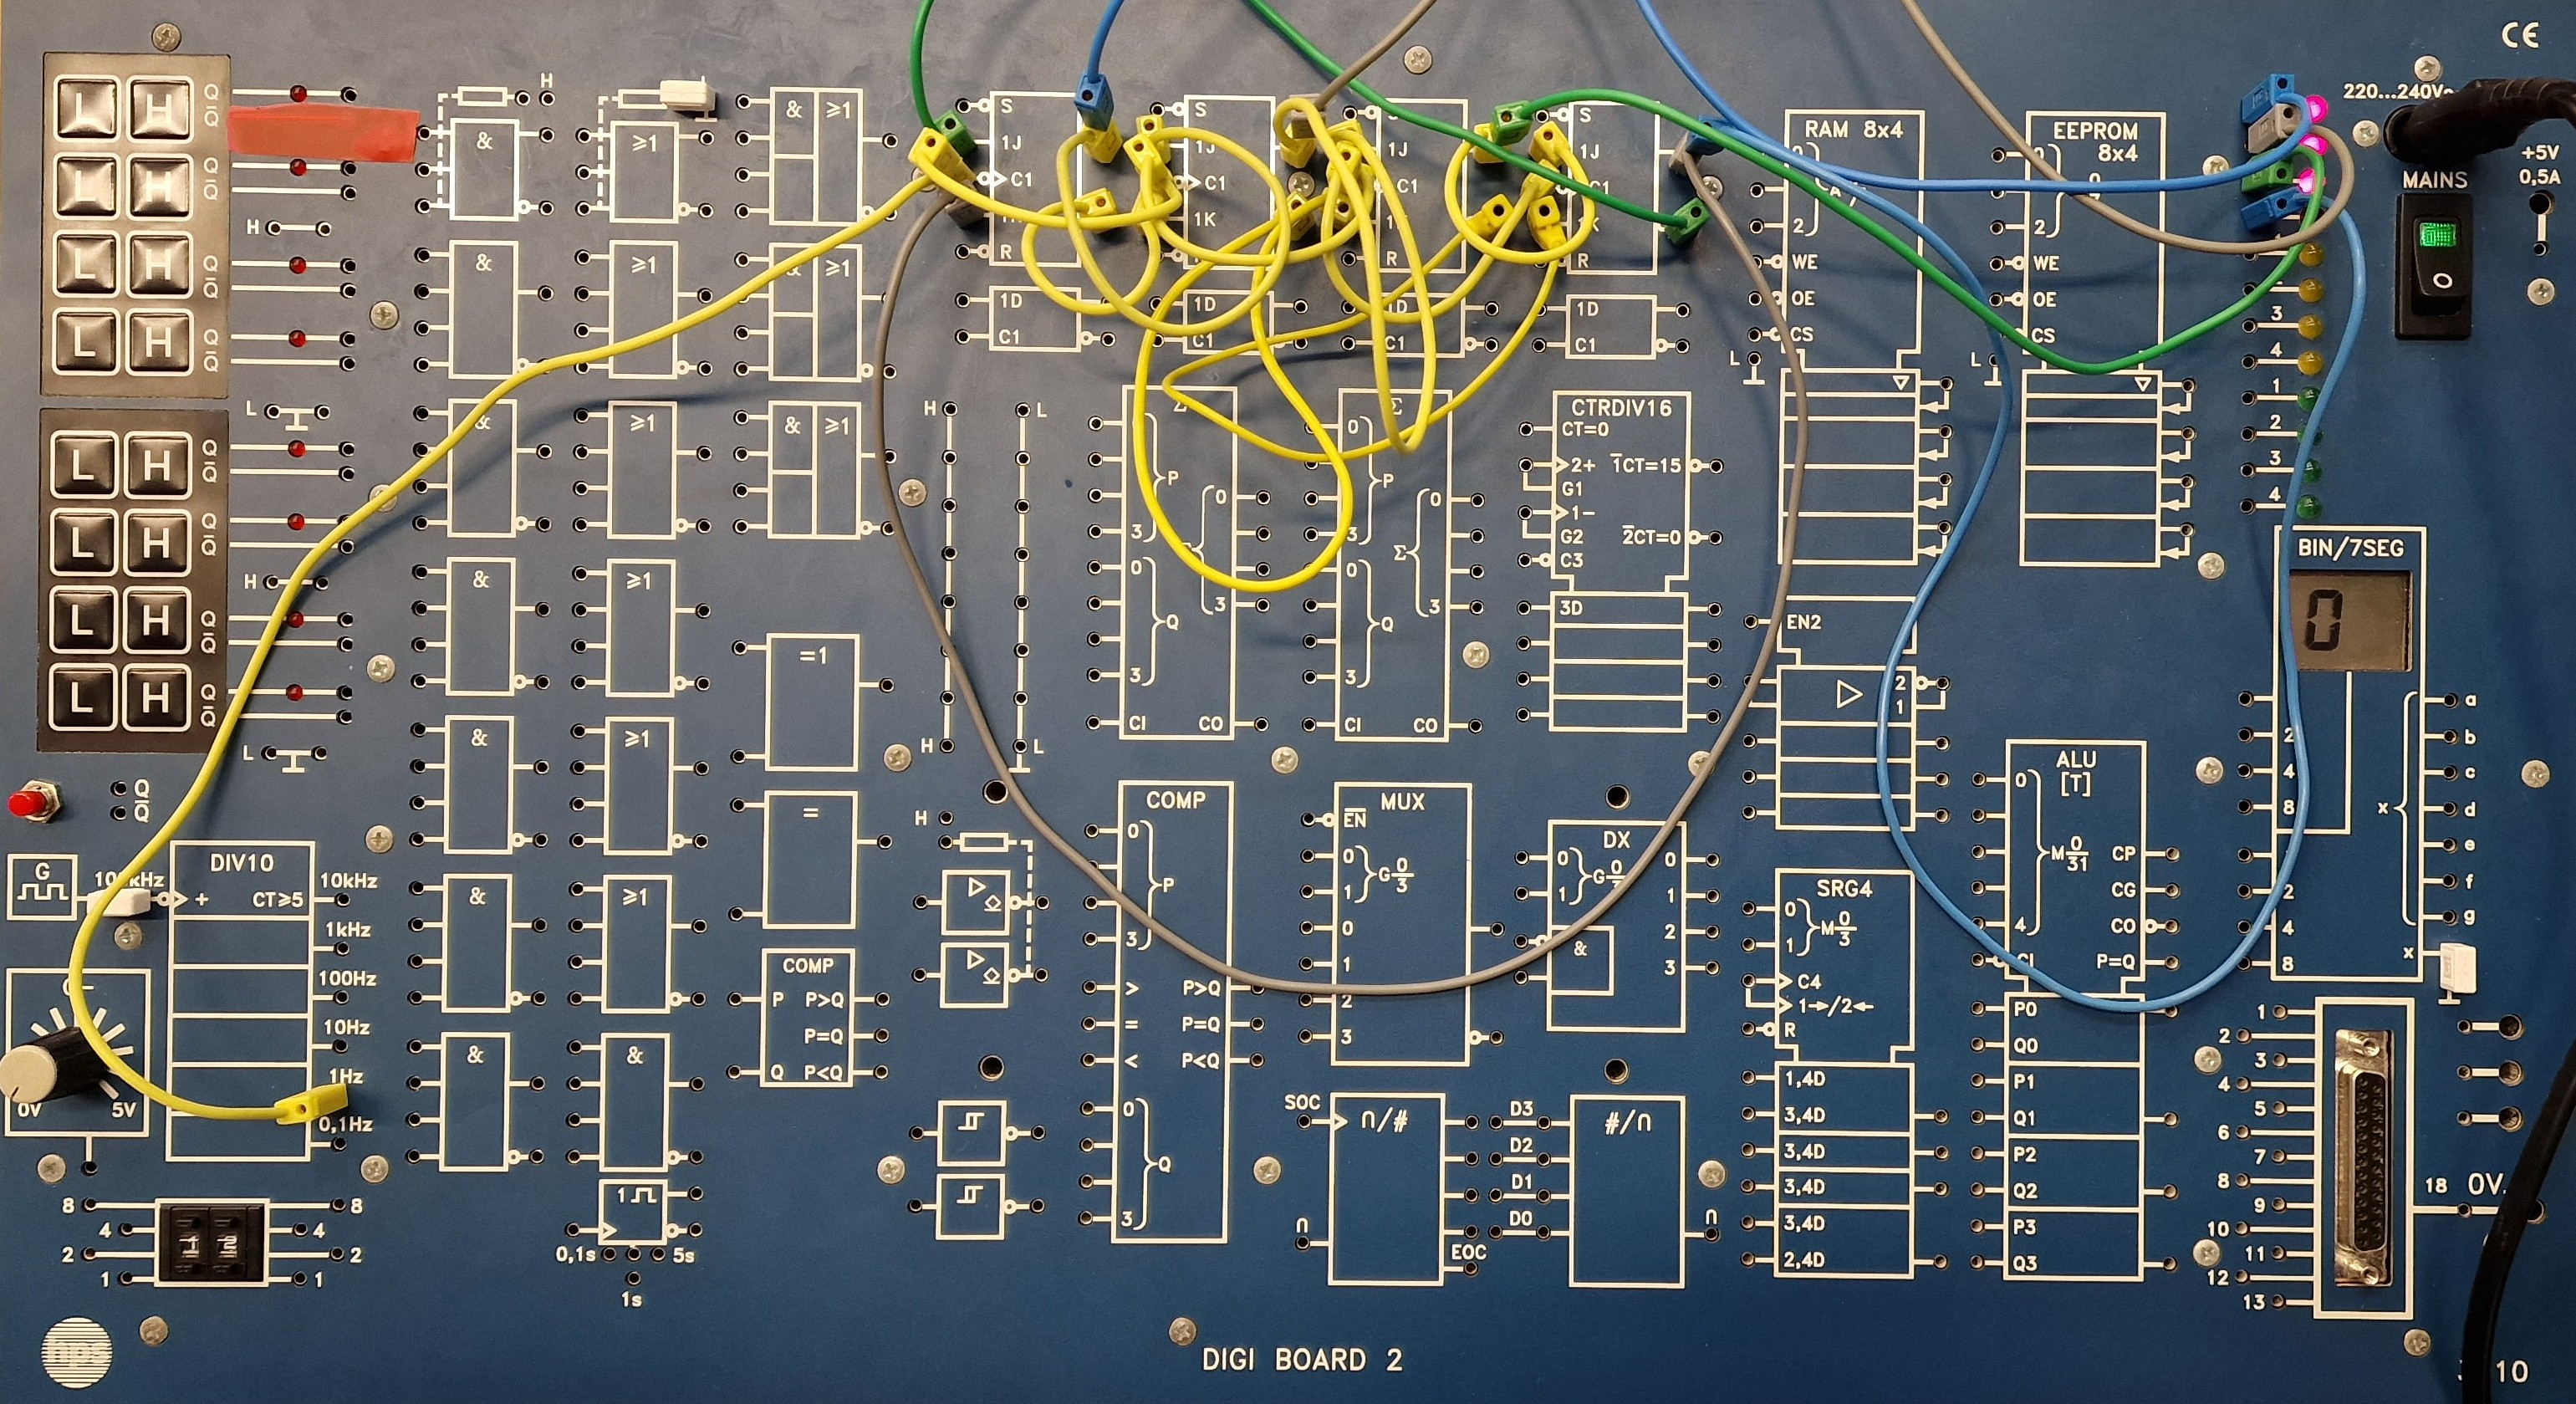
\includegraphics[width=0.8\textwidth]{1jc3.jpg}
    \caption{Gebouwde logische schakeling van twisted ring counter.}
    \label{fig:john113}
\end{figure} 
De output snoeren zijn aangesloten aan LED's en de klokingang is aangesloten aan de DIV10 blokgolf-generator.
\subsection{Controleer of de schakeling alle toestanden doorloopt}
Alle toestand zijn gecontroleerd tijdens het practicum en kwamen overeen met de toestanden die zijn aangegeven in H\ref{lol2}.
\pagebreak
\subsection{Eigenschappen en tijdvolgordediagram}
De Johnsonteller wordt in veel digitale systemen toegepast vanwege de volgende unieke eigenschappen:
\begin{itemize}
    \item De Johnsonteller verbruikt minimale energie, omdat er bij elke klokpuls maar een J-K-flip-flop veranderd van toestand;
    \item De Johnsonteller heeft 2N toestanden. Dit betekent dat er acht verschillende combinaties mogelijk zijn \cite{schuifregister}.
\end{itemize}
Zie hieronder de tijdvolgordediagram van de Johnsonteller:
\begin{figure}[h]
    \centering
    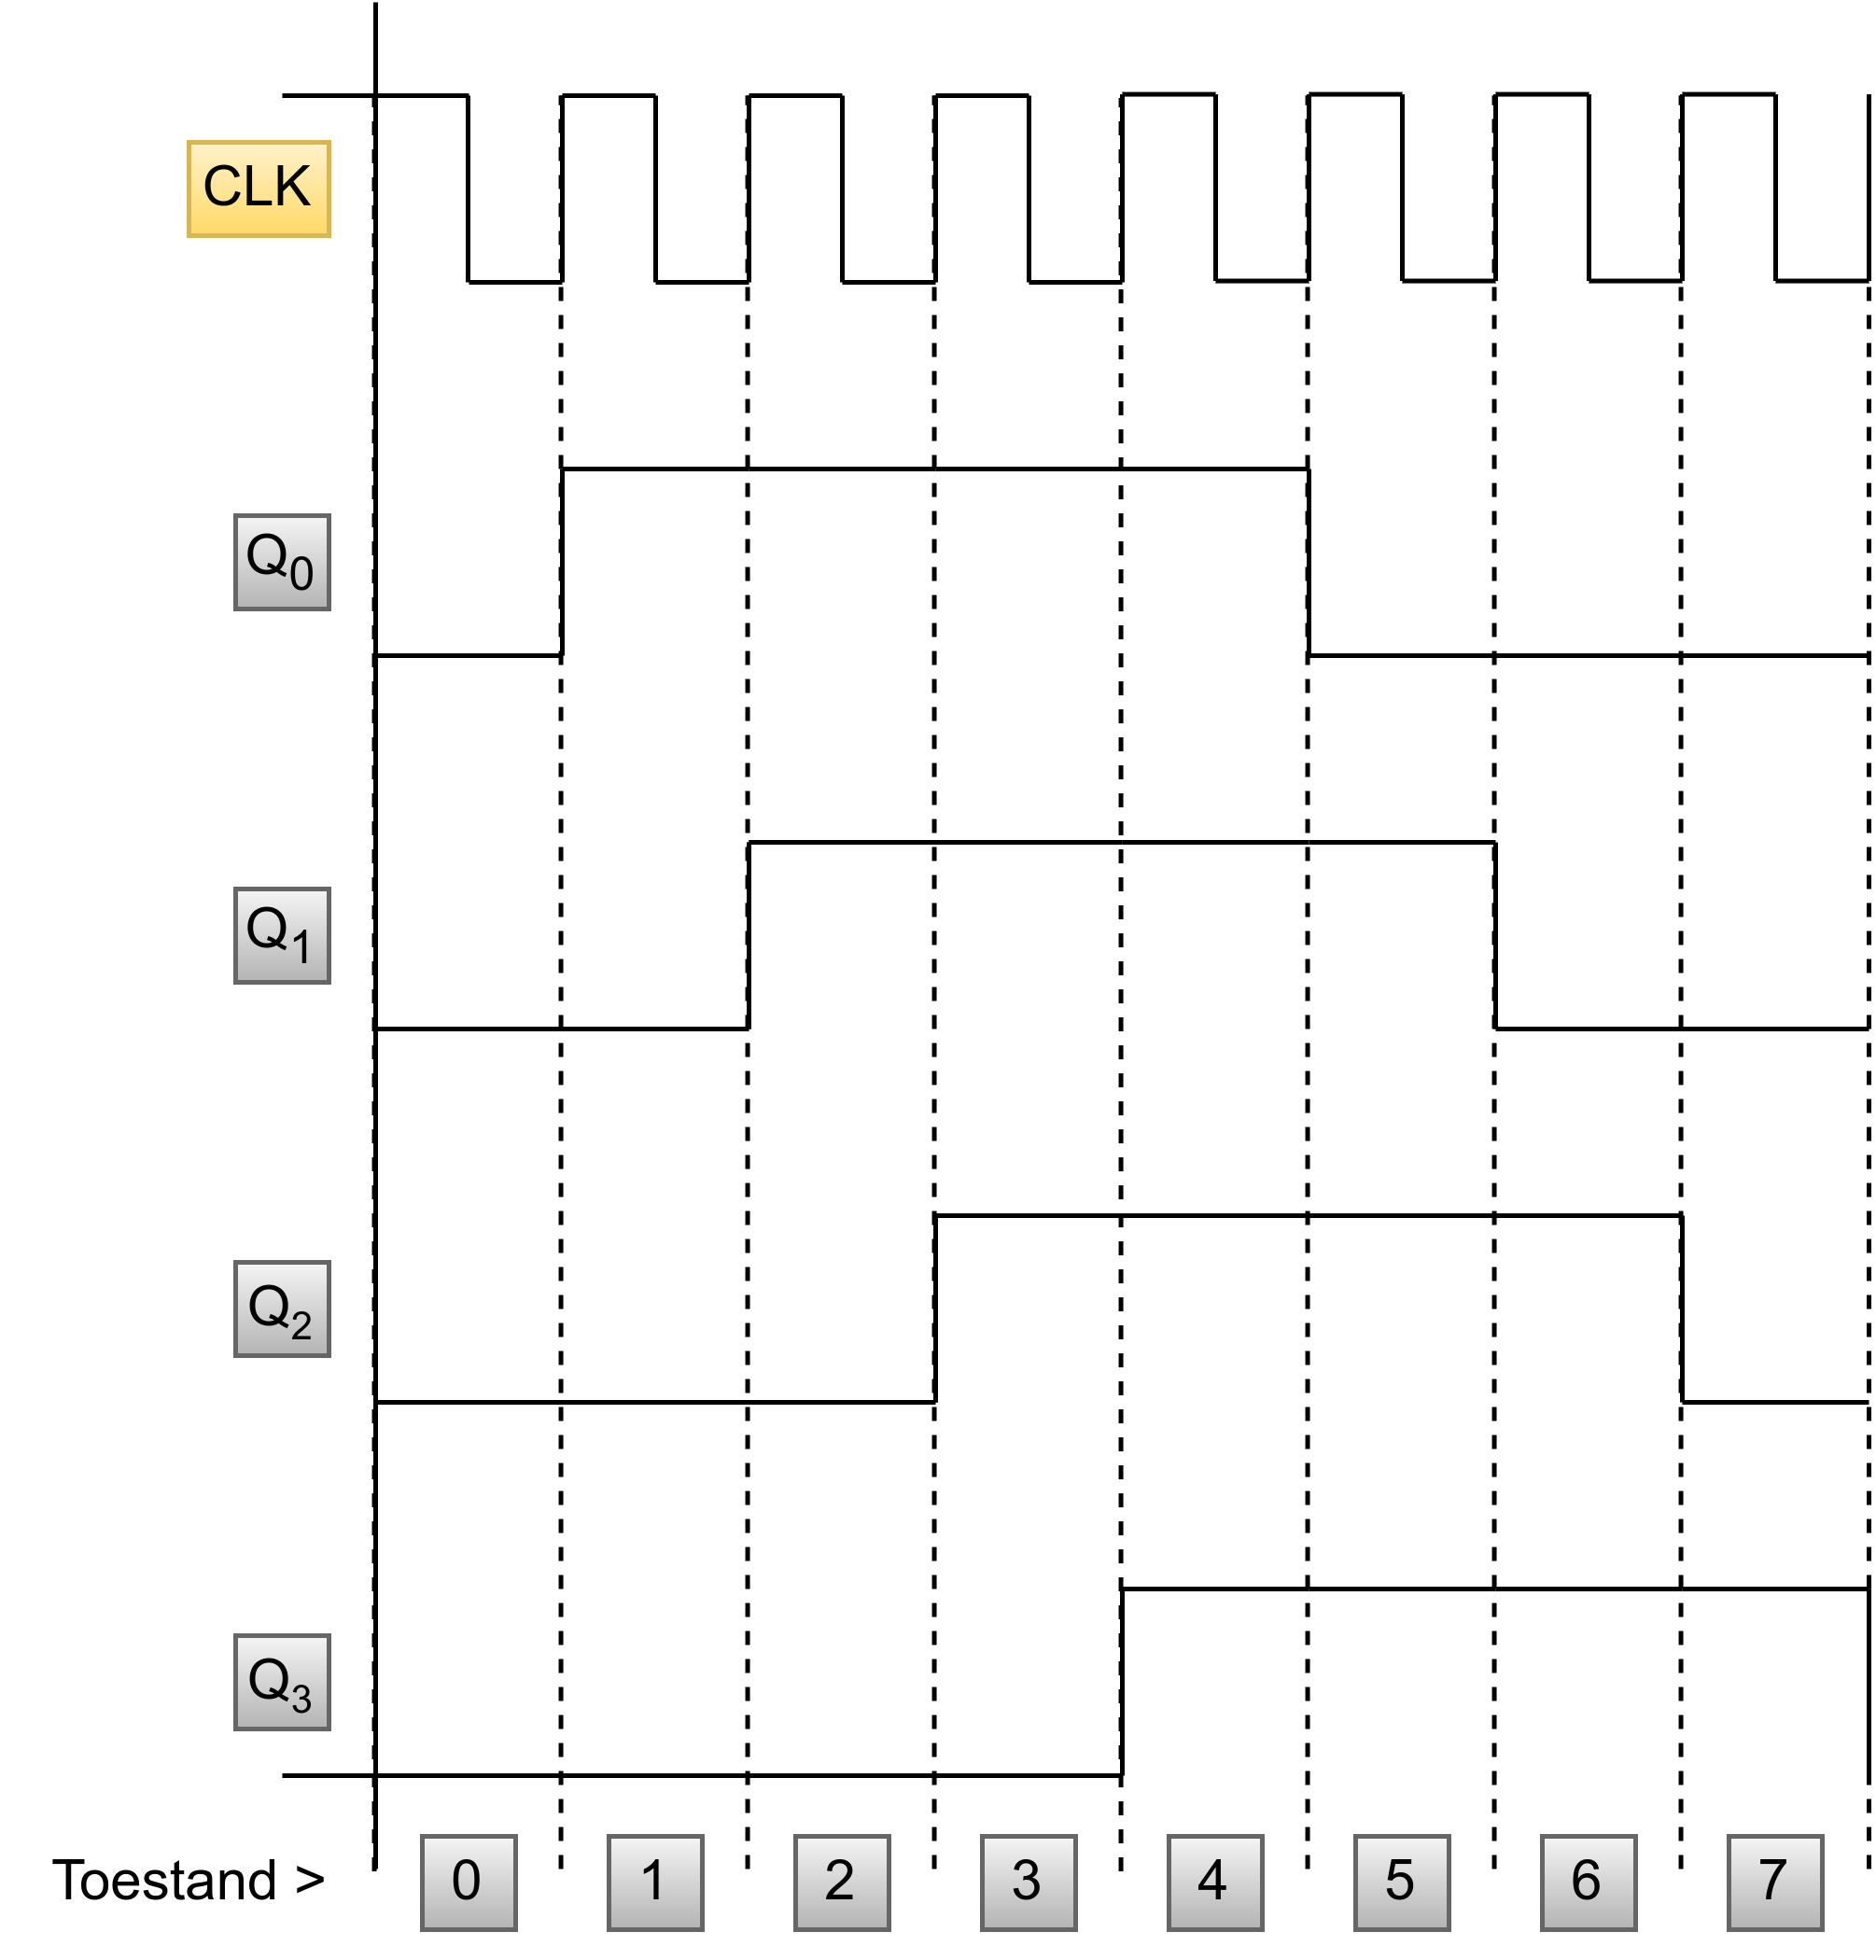
\includegraphics[width=0.5\textwidth]{tijd2.png}
    \caption{Tijdvolgordediagram van de Johnsonteller.}
    \label{fig:johsn113}
\end{figure} 
\pagebreak
\section{Teller (N-toestanden)}
In de vierde opdracht zijn de volgende deelvragen onderzocht en beantwoord over de teller met N-toestanden:
\begin{enumerate}
    \item Ontwerp met behulp van 4 J-K-flip-flops een teller met N-toestanden;
    \item Stel aan de hand van het ontwerp, de bijbehorende toestandstabel op;
    \item Hoe wordt deze teller ook wel genoemd;
    \item Bouw deze schakeling op het digiboard;
    \item Sluit de uitgang van elke flip-flop aan op een LED;
    \item Sluit op de klokingang van de J-K-flip-flops een blokgolf met een frequentie van 1 Hz aan (gebruik hiervoor de DIV 10 generator die zich op het digiboard bevindt);
    \item Wat gebeurt er;
    \item Hoe zorgen we ervoor dat de teller start;
    \item Controleer of de schakeling alle toestanden doorloopt;
    \item Eigenschappen en tijdvolgordediagram.
\end{enumerate}
\pagebreak
\subsection{Ontwerp met behulp van 4 J-K-flip-flops een teller met N-toestanden}
\begin{figure}[h]
    \centering
    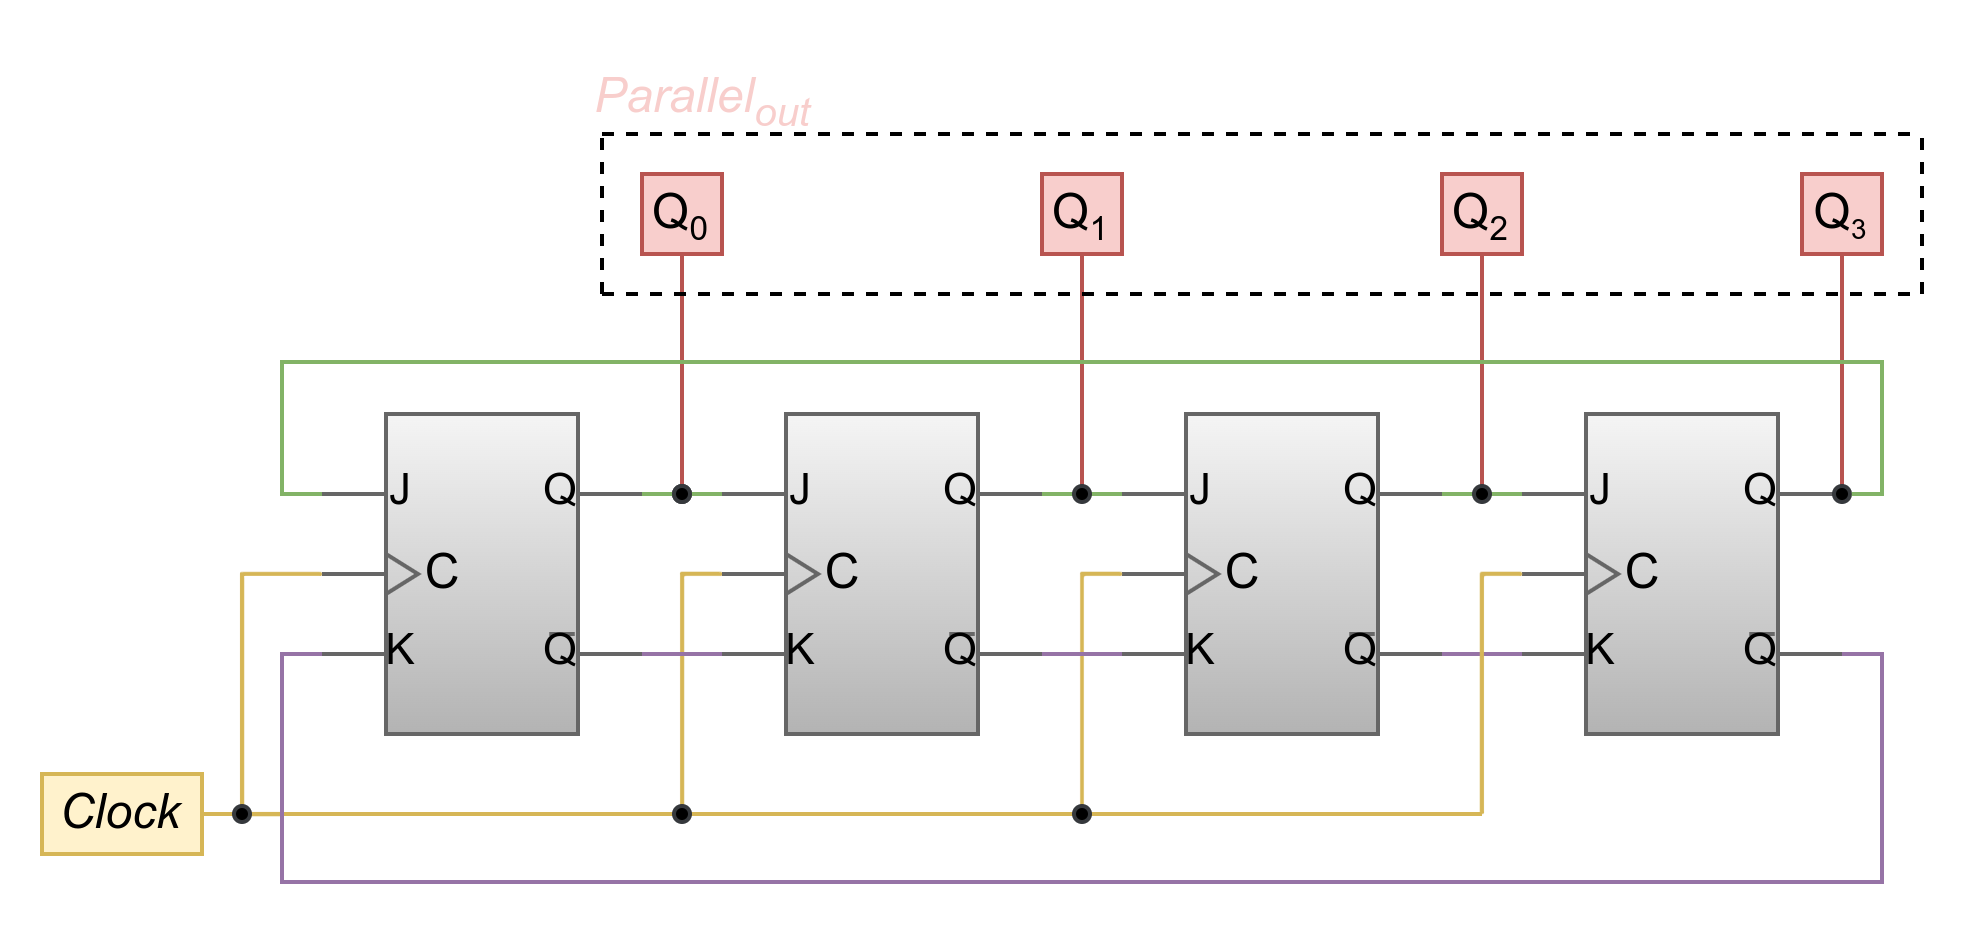
\includegraphics[width=0.8\textwidth]{ring.png}
    \caption{Logische schakeling van de N Teller.}
    \label{fig:ring}
\end{figure} 
\subsection{Stel aan de hand van het ontwerp, de bijbehorende toestandstabel op}
\label{lol}
De ringteller heeft N toestanden, dat betekent dat er maximaal vier mogelijke toestanden zijn (0 tot en met 3) \cite{1lol}. 
Zie hieronder de bijbehorende toestandstabel van de (straight) ringteller:
\begin{table}[h]
    \centering
\begin{tabular}{|lllll|}
\hline
\multicolumn{5}{|c|}{\textbf{Straight ring counter}}                                                                                                 \\ \hline
\multicolumn{1}{|l|}{\textbf{Toestand}} & \multicolumn{1}{l|}{$Q_0$} & \multicolumn{1}{l|}{$Q_1$} & \multicolumn{1}{l|}{$Q_2$} & $Q_3$ \\ \hline
\multicolumn{1}{|l|}{\textbf{0}} & \multicolumn{1}{l|}{\textbf{1}} & \multicolumn{1}{l|}{0}          & \multicolumn{1}{l|}{0}          & 0          \\ \hline
\multicolumn{1}{|l|}{\textbf{1}} & \multicolumn{1}{l|}{0}          & \multicolumn{1}{l|}{\textbf{1}} & \multicolumn{1}{l|}{0}          & 0          \\ \hline
\multicolumn{1}{|l|}{\textbf{2}} & \multicolumn{1}{l|}{0}          & \multicolumn{1}{l|}{0}          & \multicolumn{1}{l|}{\textbf{1}} & 0          \\ \hline
\multicolumn{1}{|l|}{\textbf{3}} & \multicolumn{1}{l|}{0}          & \multicolumn{1}{l|}{0}          & \multicolumn{1}{l|}{0}          & \textbf{1} \\ \hline
\multicolumn{1}{|l|}{\textbf{0}} & \multicolumn{1}{l|}{\textbf{1}} & \multicolumn{1}{l|}{0}          & \multicolumn{1}{l|}{0}          & 0          \\ \hline
\multicolumn{1}{|l|}{\textbf{1}} & \multicolumn{1}{l|}{0}          & \multicolumn{1}{l|}{\textbf{1}} & \multicolumn{1}{l|}{0}          & 0          \\ \hline
\multicolumn{1}{|l|}{\textbf{2}} & \multicolumn{1}{l|}{0}          & \multicolumn{1}{l|}{0}          & \multicolumn{1}{l|}{\textbf{1}} & 0          \\ \hline
\multicolumn{1}{|l|}{\textbf{3}} & \multicolumn{1}{l|}{0}          & \multicolumn{1}{l|}{0}          & \multicolumn{1}{l|}{0}          & \textbf{1} \\ \hline
\multicolumn{1}{|l|}{\textbf{0}} & \multicolumn{1}{l|}{\textbf{1}} & \multicolumn{1}{l|}{0}          & \multicolumn{1}{l|}{0}          & 0          \\ \hline
\end{tabular}
\end{table}
\pagebreak
\subsection{Hoe wordt deze teller ook wel genoemd}
Deze teller wordt ook wel de ``straight ring counter'' genoemd. Deze naam is gegeven omdat deze ring teller geen ``twist'' heeft, maar omdat alle flip-flops op dezelfde wijze met input en output aangesloten zijn.
\begin{figure}[h]
    \centering
    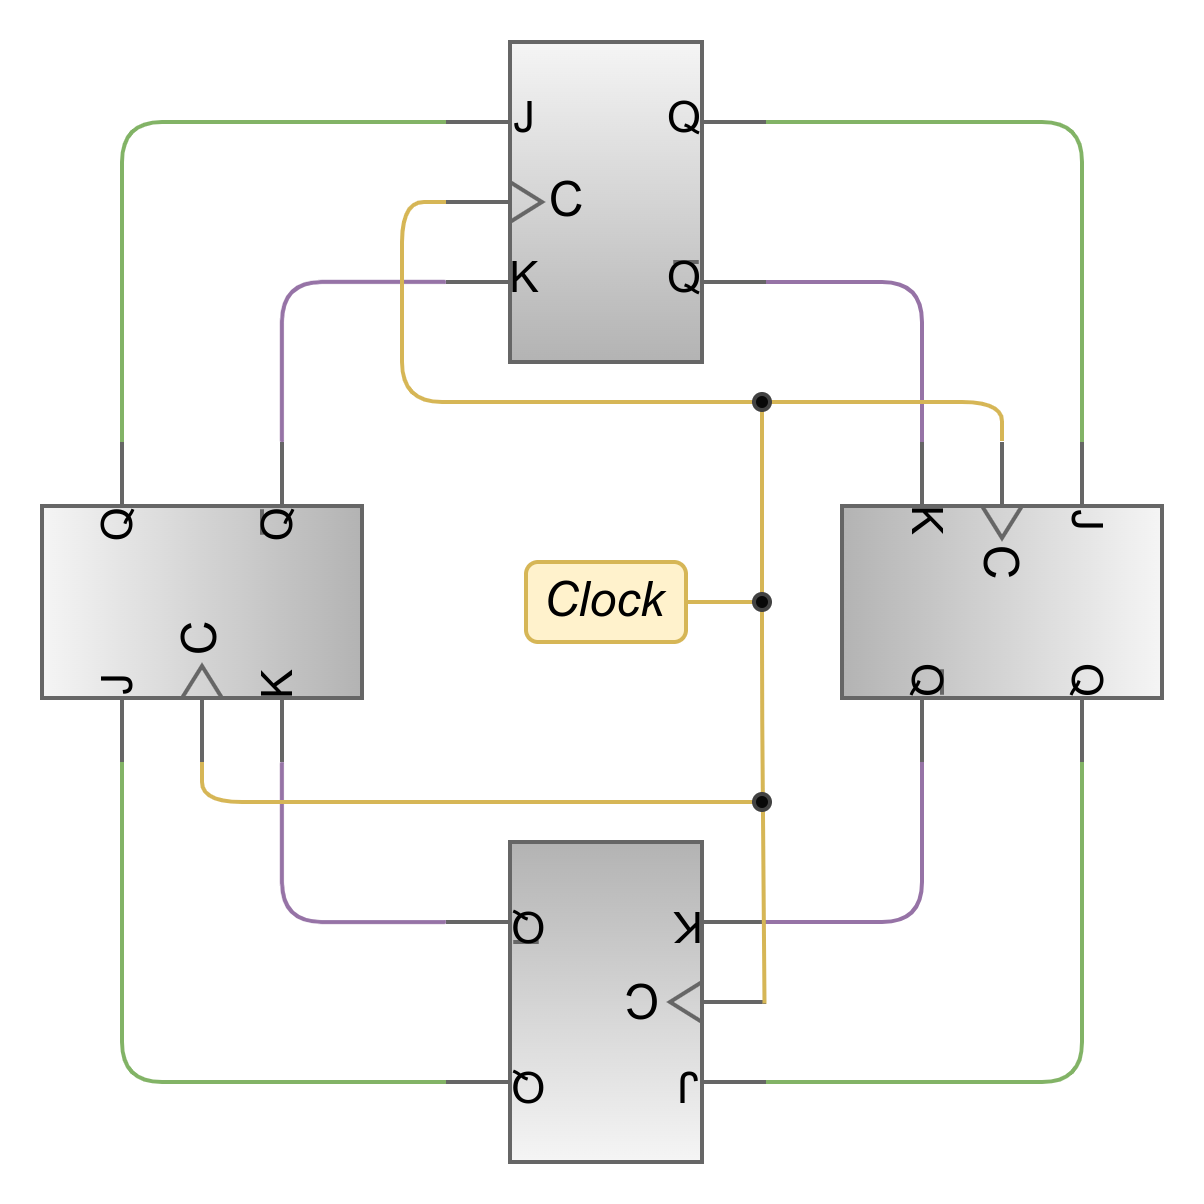
\includegraphics[width=0.8\textwidth]{ringring.png}
    \caption{Logische schakeling van straight ring counter.}
    \label{fig:ringring}
\end{figure}
\pagebreak
\subsection{Bouw deze schakeling op het digiboard}
\begin{figure}[h]
    \centering
    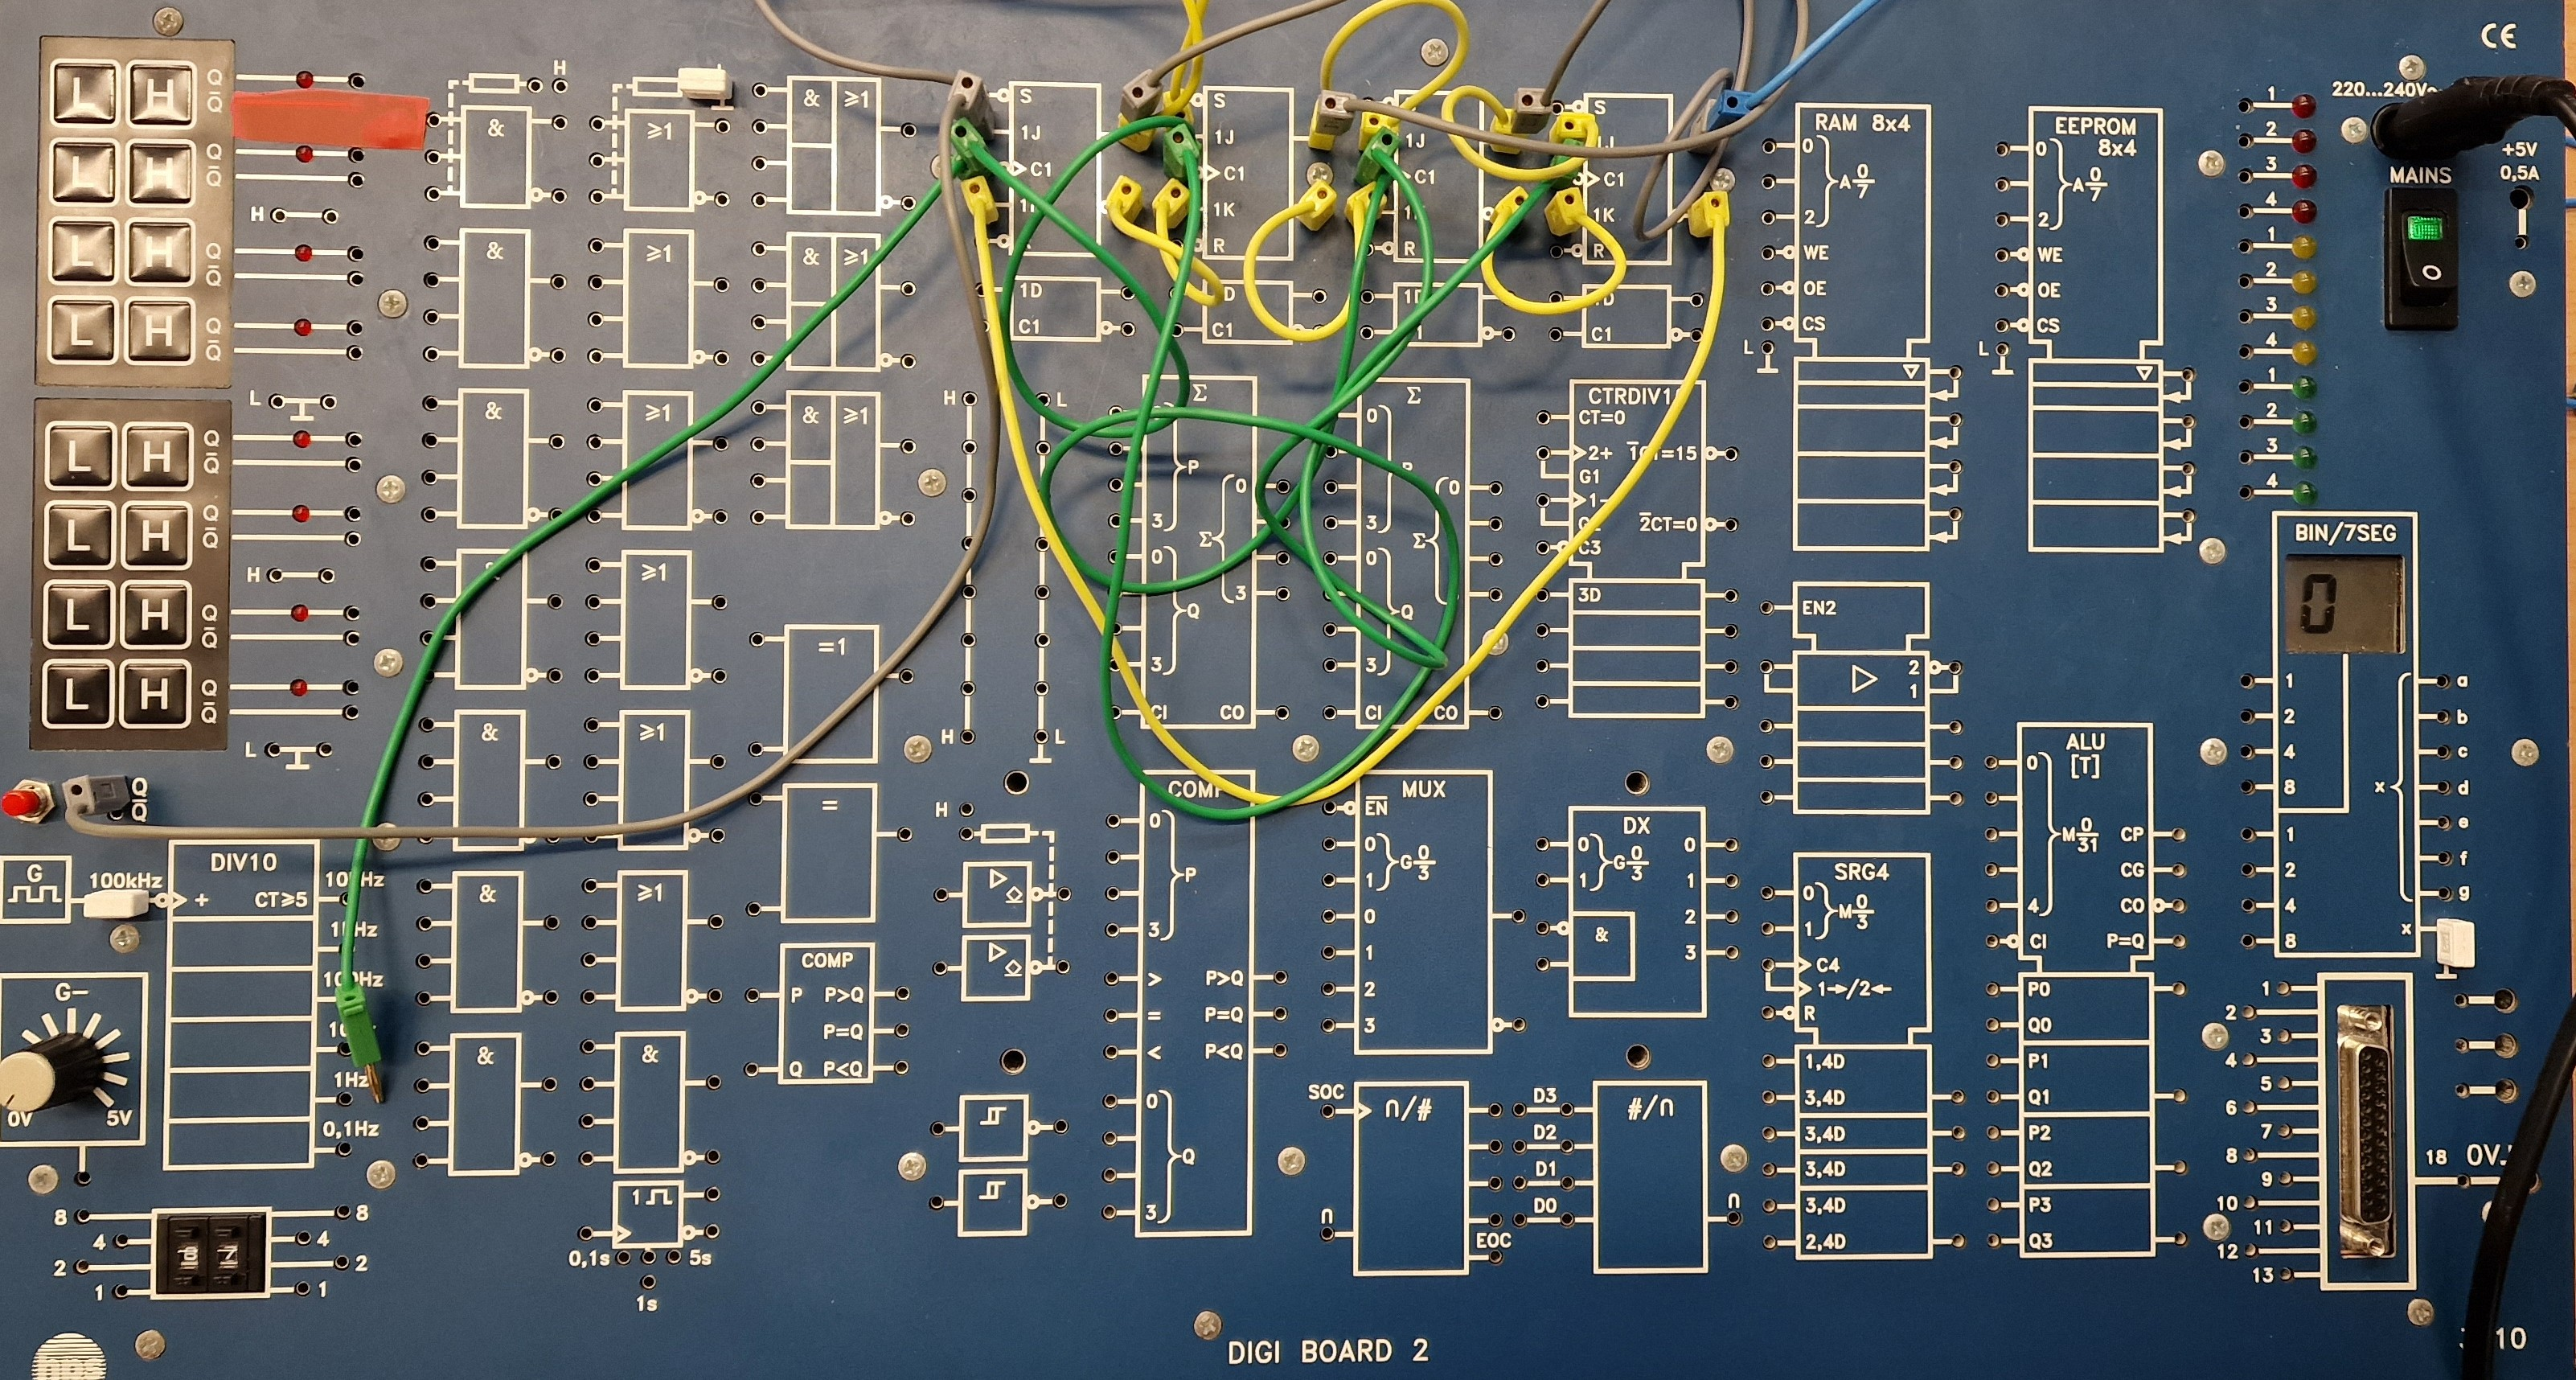
\includegraphics[width=0.7\textwidth]{1ringstraight.jpg}
    \caption{Gebouwde logische schakeling van straight ring counter.}
    \label{fig:rs}
\end{figure} 
\subsection{Sluit de uitgang van elke flip-flop aan op een LED}
\begin{figure}[h]
    \centering
    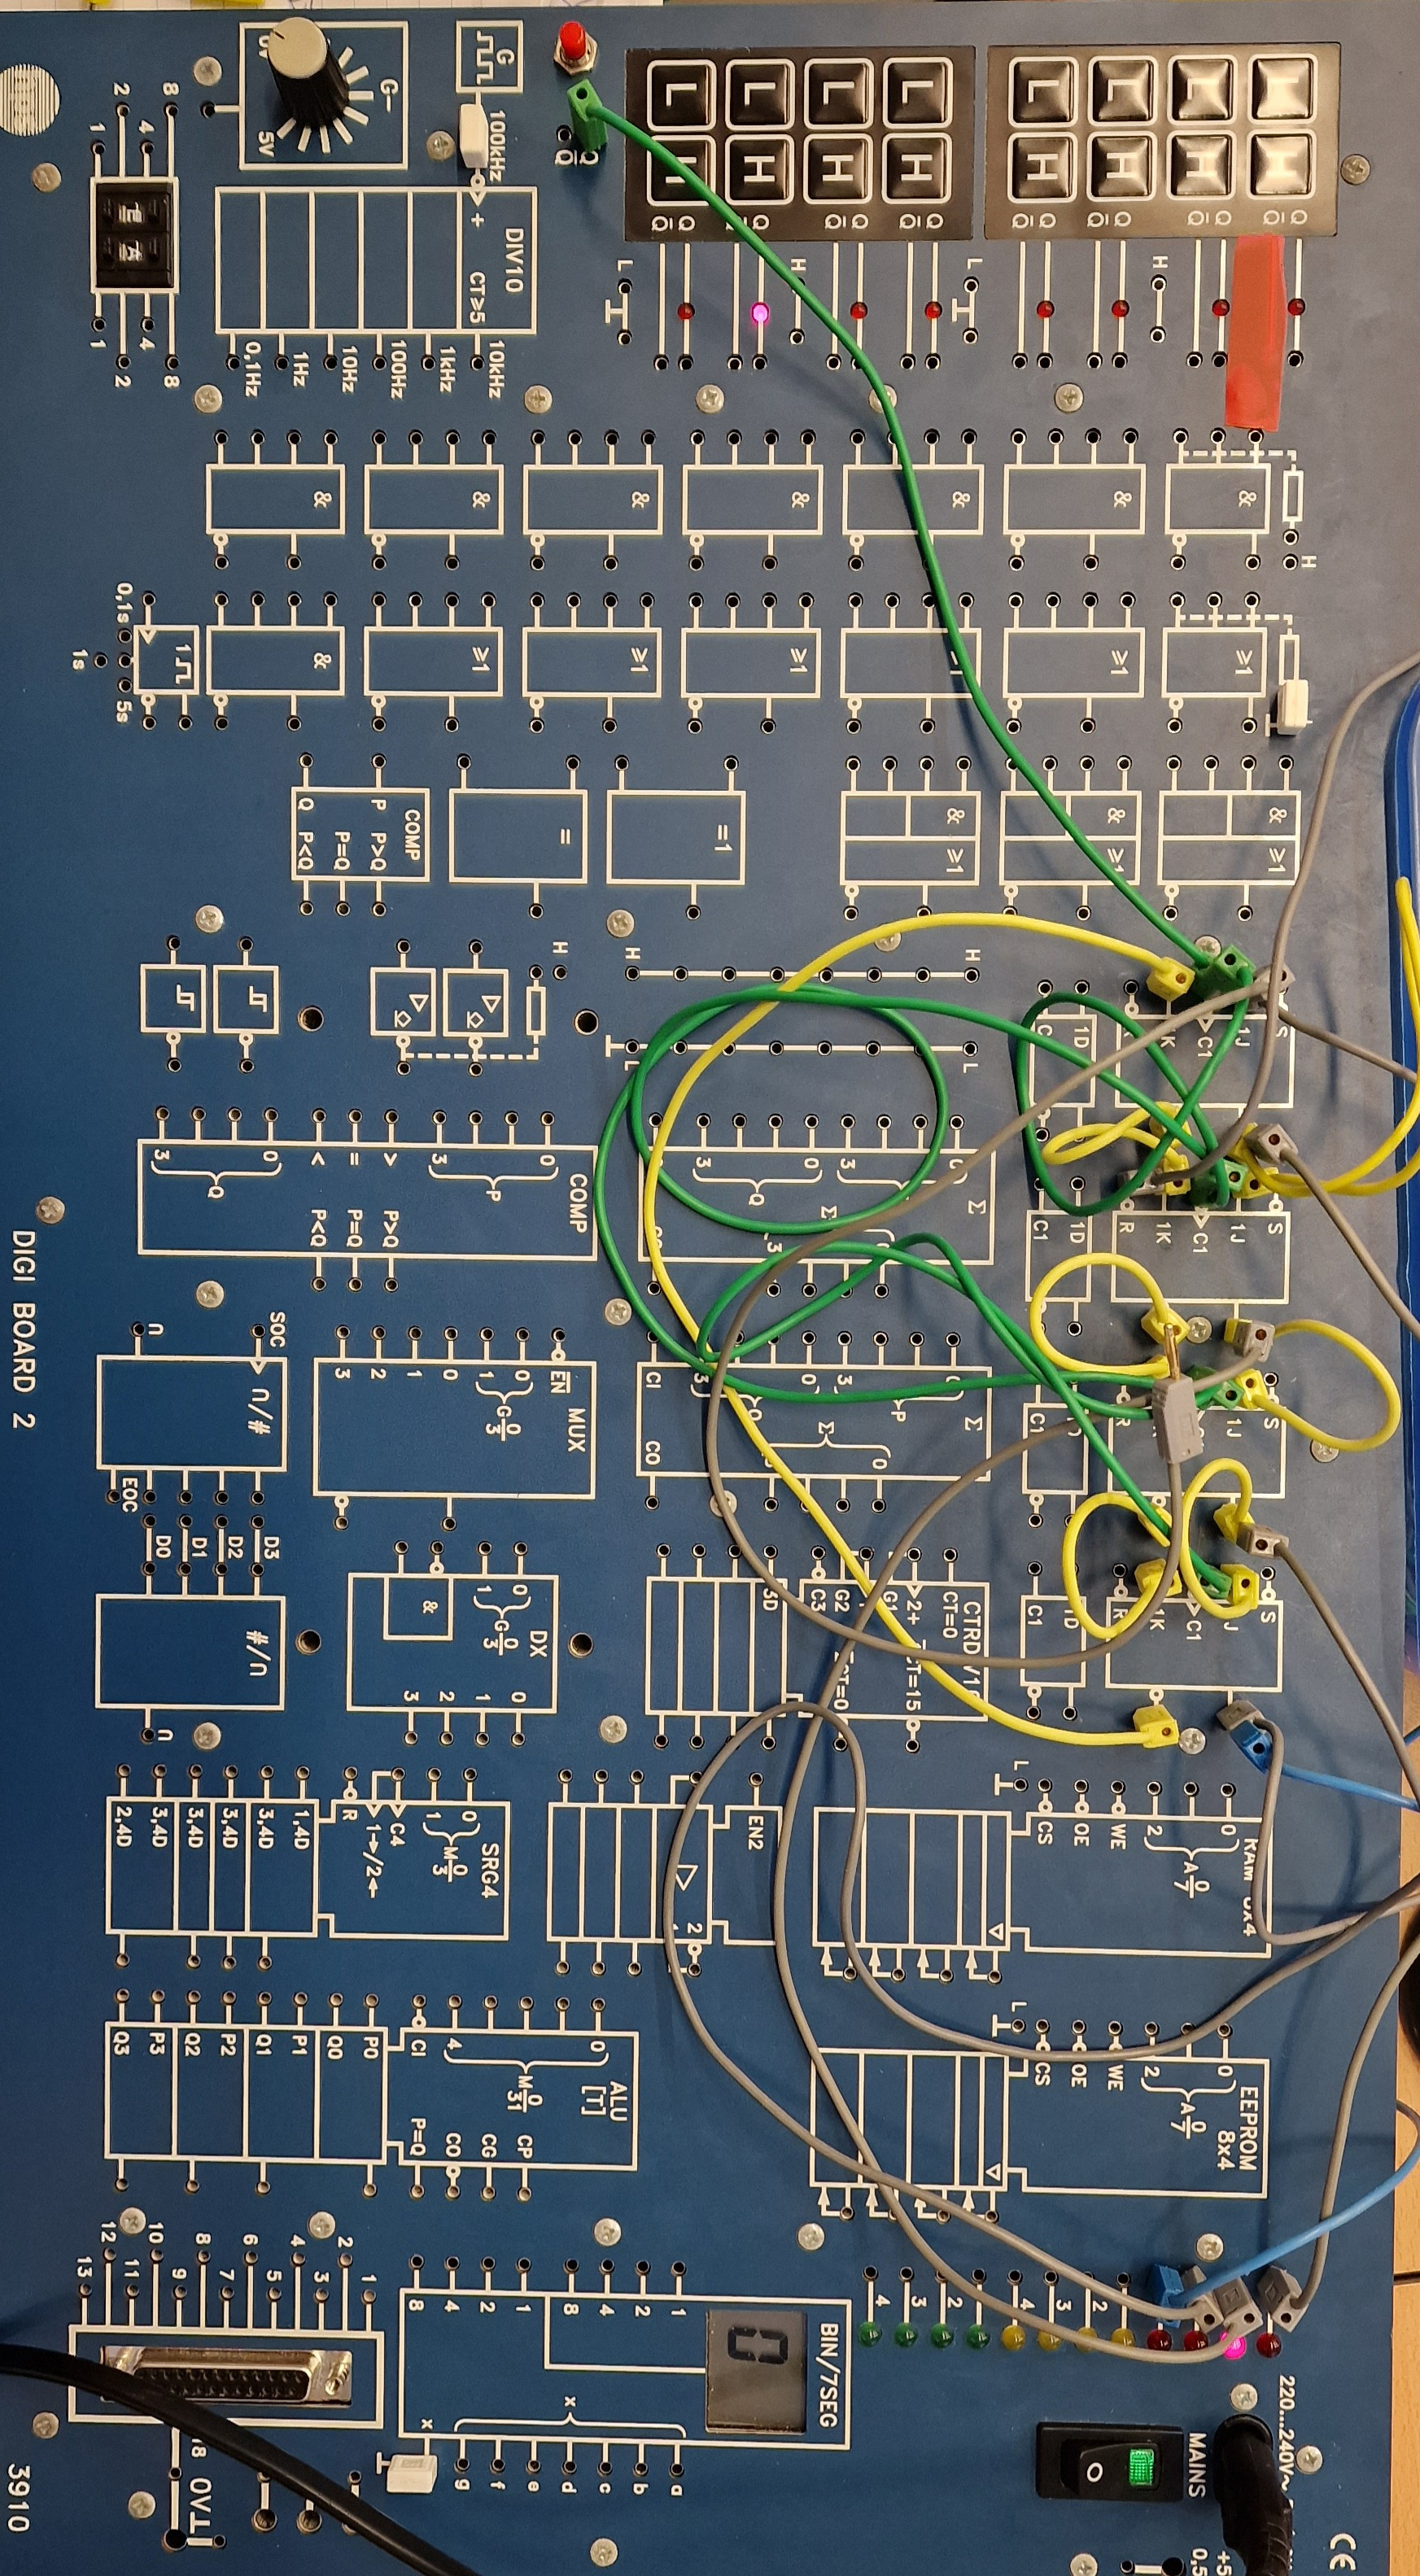
\includegraphics[angle=90,width=0.7\textwidth]{1ring.jpg}
    \caption{Gebouwde logische schakeling van straight ring counter.}
    \label{fig:rs}
\end{figure} 
Hierbij zijn de output snoeren aangesloten aan LED's.
\pagebreak
\subsection{Sluit op de klokingang van de J-K-flip-flops een blokgolf met een frequentie van 1 Hz aan}
\begin{figure}[h]
    \centering
    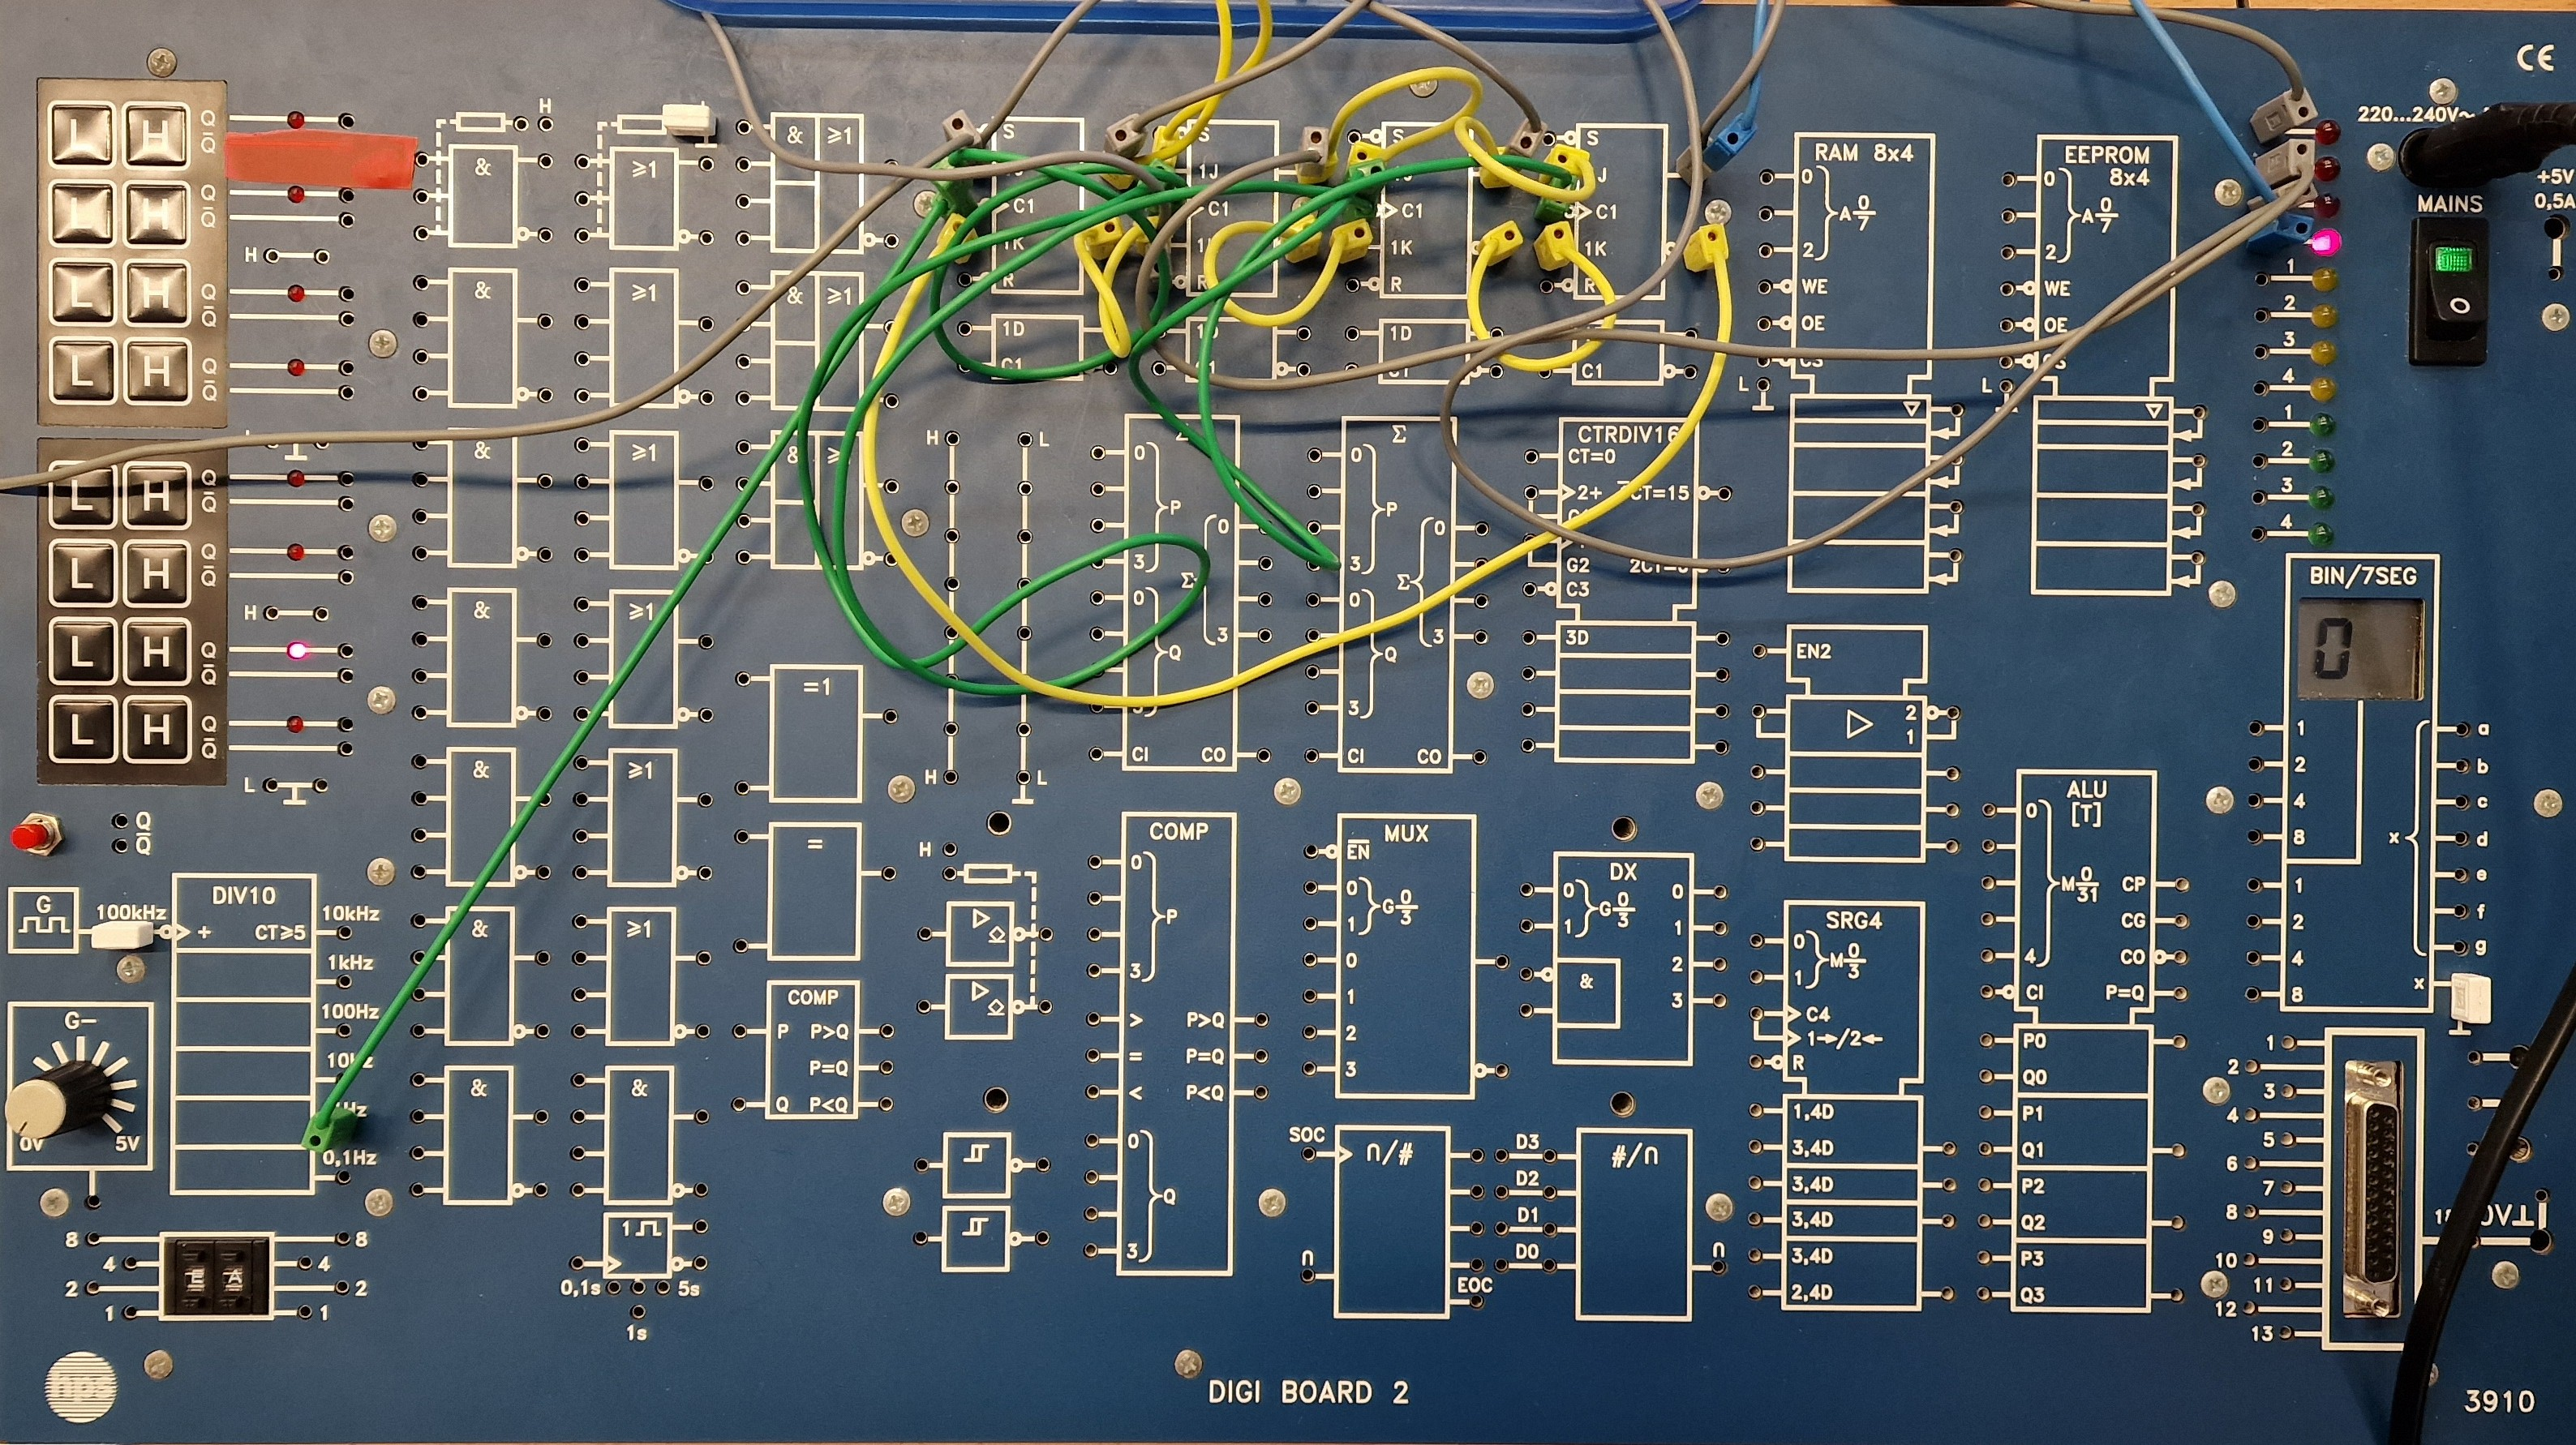
\includegraphics[width=0.8\textwidth]{1rsaan.jpg}
    \caption{Gebouwde logische schakeling van straight ring counter.}
    \label{fig:rsaan}
\end{figure} 
Hierbij zijn de output snoeren aangesloten aan LED's. Ook is de klokingang aangesloten aan de DIV10 blokgolf-generator met een frequentie van 1 Hz.
\subsection{Wat gebeurt er}
De straight ring counter gaat met een frequentie van 1 Hz door alle toestanden heen. 
\subsection{Hoe zorgen we ervoor dat de teller start}
Eerst moet de eerste J-K-flip-flop geladen worden met een korte actief-hoge puls, daarna kan de klok geactiveerd worden. Nu zal de ring teller ervoor zorgen dat die actief-hoge puls doorgevoerd zal worden naar de volgende toestand, zoals beschreven in de toestandstabel.
\subsection{Controleer of de schakeling alle toestanden doorloopt}
De toestanden waren tijdens het practicum gecontroleerd en werkte de teller succesvol. 
Alle toestanden kwamen precies overeen zoals gerepresenteerd in H\ref{lol}.
\pagebreak
\subsection{Eigenschappen en tijdvolgordediagram}
De ringteller heeft de volgende eigenschappen:
\begin{itemize}
    \item De ringteller kan niet zelf starten. Dit houdt in dat er in eerste instantie een actief-hoge puls geladen moet worden door een van de J-K-flip-flop's;
    \item De ringteller heeft N toestanden. Dit betekent dat er vier verschillende combinaties mogelijk zijn \cite{schuifregister}.
\end{itemize}
Zie hieronder de tijdvolgordediagram van de ringteller:
\begin{figure}[h]
    \centering
    \includegraphics[width=0.3\textwidth]{tijd1.png}
    \caption{Tijdvolgordediagram van de ringteller.}
    \label{fig:johssn113}
\end{figure} 
\pagebreak
\section{Conclusie}
\label{Conclusie}
In dit verslag is er onderzoek gedaan naar de werking van de multiplexer, de BCD-encoder, straight ring counter en de twisted ring counter (Johnson counter). 
Daarbij was ook een probleemstelling geïntroduceerd in H\ref{Problem} en de bijbehorende doelstellingen, zie hieronder:
\begin{enumerate}
    \item Inzicht te verkrijgen in logische functies die ten grondslag liggen aan de digitale techniek;
    \item Waarnemingen te verrichten aan de bijbehorende eenvoudige logische schakelingen;
    \item De bijbehorende meetgegevens en waarheidstabellen op een juiste wijze te verkrijgen en te interpreteren;
    \item De vergaarde gegevens te verwerken tot een verslag.
\end{enumerate}
De probleemstelling was:
\begin{itemize}
    \item \textit{``Inzicht krijgen in de werking van een aantal complexe logische schakelingen en daarna deze op een efficiënte wijze te ontwerpen en te bouwen?''}
\end{itemize}

Bij de eerste practicumopdracht \textit{``Combinatorische logische functie: MUX''} werd geëxperimenteerd met een 4-bit multiplexer. 
Hierbij was de opdracht om een logische schakeling te ontwerpen en te bouwen dat ervoor zorgt dat er 4-bits aan data-lijnen gekozen kunnen worden door middel van 2-bits data-select-lijnen.
Om dat te kunnen doen is er gebruik gemaakt van een waarheidstabel en een SOP-expressie. 
De bijbehorende logische schakelingen zijn allemaal gebouwd, getest en gecontroleerd op de werking ervan. 

Vervolgens is er in de tweede practicumopdracht \textit{``Combinatorische logische functie: BCD-encoder''} geëxperimenteerd met een Binary-Coded-Decimal encoder. 
Deze encoder heeft als functie dat de decimale input met getallen van 0 tot en met 9 wordt omgezet in binaire code, dus daarom is het daarnaar vernoemd. 
Tijdens het testen van de logische schakeling kwamen we erachter dat het getal `0' niet een input knop heeft, omdat het getal `0' in binair ``0000'' is. 
De output was aangesloten aan de BCD-decoder van het digiboard en die vertaalde dat gelukkig automatisch naar `0'.   
Voor de rest werkte de logische schakelingen zoals vanuit de theorie verwacht was, en waren er geen andere problemen. 
De werking van de encoder is hieronder nog gerepresenteerd:
\pagebreak
\begin{figure}[h]
    \centering
    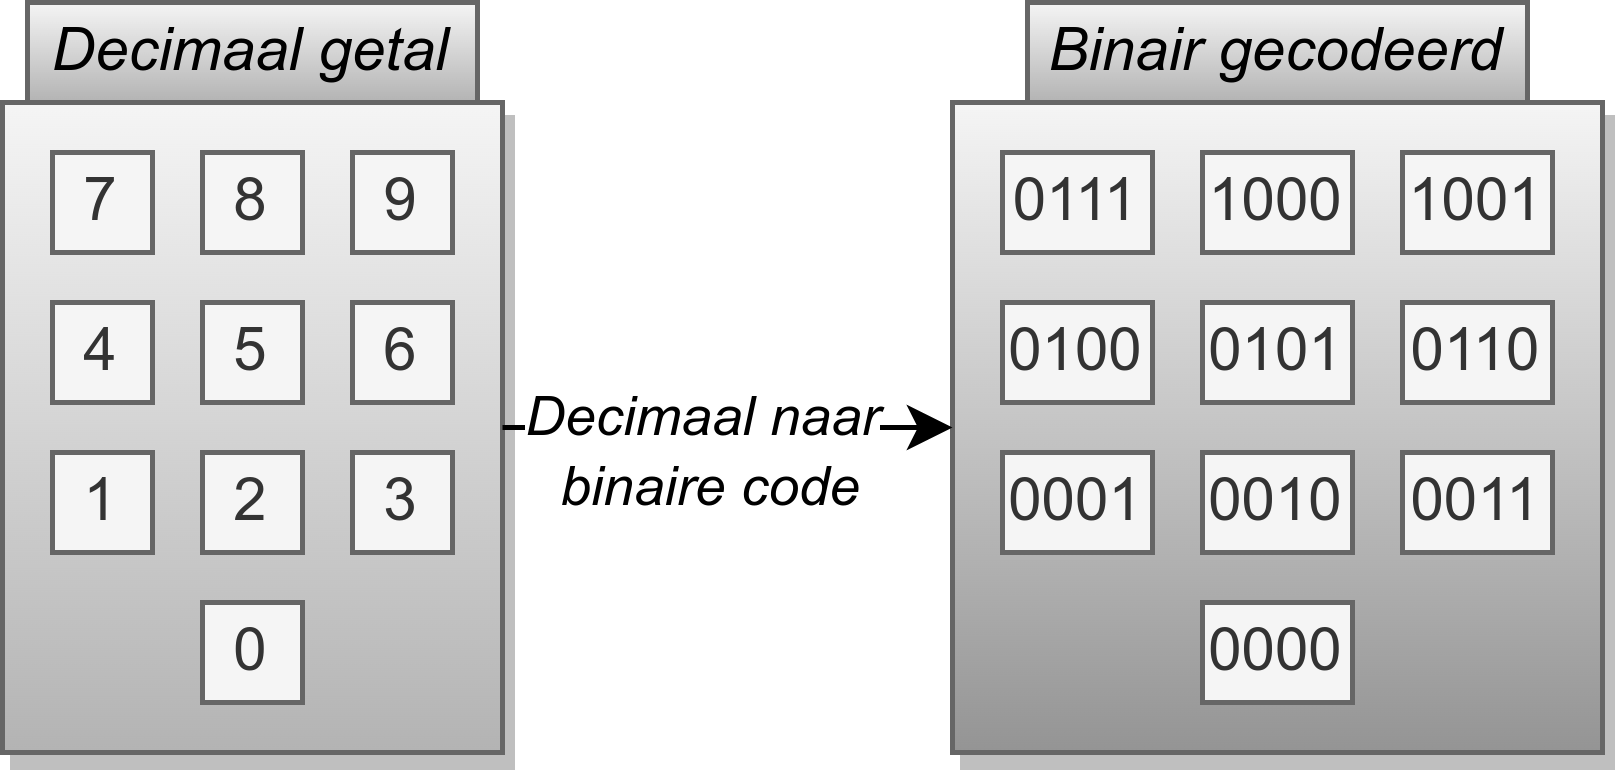
\includegraphics[width=0.5\textwidth]{conc.png}
    \caption{Abstracte blokschema dat de werking van de BCD-encoder representeert.}
    \label{fig:rds}
\end{figure} 

In de derde practicumopdracht \textit{``Teller (2N-toestanden)''} is er geëxperimenteerd met een twisted ringteller ook wel bekend als de Johnson counter. 
Deze schakeling maakt gebruik van vier J-K-flip-flop's: de klokingangen zijn allemaal aangesloten aan dezelfde klokgenerator, de `Q' output van de laatste J-K-flip-flop is verbonden aan K van de eerste J-K-flip-flop en hetzelfde principe geldt ook voor $\overline{Q}$ naar input J. 
De Johnsonteller wordt in veel digitale systemen toegepast vanwege de volgende unieke eigenschappen:
\begin{itemize}
    \item De Johnsonteller verbruikt minimale energie, omdat er bij elke klokpuls maar een J-K-flip-flop veranderd van toestand;
    \item De Johnsonteller heeft 2N toestanden. Dit betekent dat er acht verschillende combinaties mogelijk zijn.
\end{itemize}
De Johnsonteller schakelt dus snel, omdat de teller werkt in een éénwisselcode. De alternatieve naam ``twisted ring counter'' komt van het feit dat de logische schakelingen een ``ring'' als structuur heeft. Daarnaast bevat de schakeling een ``twist'', dus vandaar ``twisted ring counter''. 

Bij de laatste opdracht \textit{``Teller (N-toestanden)''} is er geëxperimenteerd met een straight ring counter ook wel bekend als de ringteller. 
Deze schakeling maakt gebruik van vier J-K-flip-flop's: de klokingangen zijn allemaal aangesloten aan dezelfde klokgenerator, de J ingangen en uitgangen zijn allemaal doorgelust aan elkaar en de K ingangen en uitgangen zijn ook allemaal doorgelust aan elkaar. 
De ringteller heeft de volgende eigenschappen:
\begin{itemize}
    \item De ringteller kan niet zelf starten. Dit houdt in dat er in eerste instantie een actief hoge puls geladen moet worden door een van de J-K-flip-flop's;
    \item De ringteller heeft N toestanden. Dit betekent dat er vier verschillende combinaties mogelijk zijn.
\end{itemize}
Deze ringteller wordt voornamelijk toegepast in sequentiële systemen, omdat deze tellers tijdbepalende pulsen kunnen genereren. 



De bovenstaande probleemstelling is dan ook op een succesvolle wijze opgelost door:
\begin{enumerate}
    \item Eerst een waarheidstabel te maken van de toegepaste logische schakeling. Hiermee worden alle Booleaanse mogelijkheden op een overzichtelijke manier gerepresenteerd;
    \item Als tweede stap is op basis van de waarheidstabel een eenvoudige Booleaanse expressie opgesteld;
    \item Als derde stap is een Karnaugh diagram gemaakt. Daarmee konden er allerlei groepjes gevormd worden van binaire getallen om de minimalisatie mogelijk te maken;
    \item Tenslotte werd een logische schakeling ontworpen en is deze gebouwd op het digiboard. Op deze gestructureerde manier is er op een effectieve manier een toegepaste logische schakeling ontworpen en gebouwd!
\end{enumerate}
Dus er kan geconcludeerd worden dat de vier doelstellingen van dit practicumverslag met succes gerealiseerd zijn!
\pagebreak






\nocite{*}
\section{Bronvermelding}

\bibliography{library.bib}
\bibliographystyle{IEEEtran}

\pagebreak
\end{document}